
\documentclass[%
 reprint,
%superscriptaddress,
%groupedaddress,
%unsortedaddress,
%runinaddress,
%frontmatterverbose, 
%preprint,
%preprintnumbers,
nofootinbib,
%nobibnotes,
%bibnotes,
 amsmath,amssymb,
 aps,
%pra,
%prb,
%rmp,
%prstab,
%prstper,
%floatfix,
]{revtex4-2}
\usepackage{gensymb}
\usepackage{textcomp}
\usepackage{graphicx}% Include figure files
\usepackage{dcolumn}% Align table columns on decimal point 


\usepackage{bm}% bold math
\usepackage{siunitx}
\sisetup{separate-uncertainty=true}
\usepackage{tabularx}
\usepackage{amssymb}
\usepackage{amsmath}
\usepackage{relsize}
\usepackage{enumitem}
\usepackage{float}
\usepackage{booktabs}
\usepackage{makecell}
\usepackage[colorlinks,bookmarks=false,citecolor=blue,linkcolor=blue,urlcolor=blue]{hyperref}
%\usepackage{hyperref}% add hypertext capabilities
%\usepackage[mathlines]{lineno}% Enable numbering of text and display math
%\linenumbers\relax % Commence numbering lines

%\usepackage[showframe,%Uncomment any one of the following lines to test 
%%scale=0.7, marginratio={1:1, 2:3}, ignoreall,% default settings
%%text={7in,10in},centering,
%%margin=1.5in,
%%total={6.5in,8.75in}, top=1.2in, left=0.9in, includefoot,
%%height=10in,a5paper,hmargin={3cm,0.8in},
%]{geometry}

\begin{document}

\preprint{APS/123-QED}

\title{Experiments with Lock-in Amplifier}% Force line breaks with \\


\author{Maitrey Sharma}
\email{maitrey.sharma@niser.ac.in}
\affiliation{School of Physical Sciences, National Institute of Science Education and Research, HBNI, Jatni-752050, India}




\date{\today}% It is always \today, today,
             %  but any date may be explicitly specified

\begin{abstract}
    In this experiment, we study about the lock-in amplifier, and its working principle, namely, phase sensitive detection. A lock-in amplifier is a special type of amplifier that can extract a signal with a known carrier wave from an extremely noisy environment, which makes it immensely useful in numerous fields with a lot of applications. We use the lock-in amplifier to perform experimental study of two separate, very important aspects of electrodynamics, namely, mutual inductance and resistances. Mutual inductance is defined as the ratio between the emf induced in one loop or coil by the rate of change of current in another loop or coil. We deduce various results related to the phenomena of mutual inductance thereafter. Further, we employ the lock-in amplifier to find value of a small resistance (less than $\SI{1}{\ohm}$). In the process of these experiments, we establish various useful results relates to magnetism and behaviour of voltage and current in magnetic fields.
\end{abstract}

\keywords{lock-in amplifier, Mutual inductance}
\maketitle

%\tableofcontents

\section{\label{sec:level1}Introduction}
    Ever since the development of audio communication technology which began when the first telephone was patented in 1876, the need to increase the amplitude of electrical signals to extend the transmission of signals over increasingly long distances also became imminent as well. Amplifiers first appeared in 1912 after Lee De Forest invented the triode vacuum tube in 1906. After the invention of transistors in 1947 at Bell Labs by John Bardeen and Walter Brattain and the developments from there changed the way how amplifiers work further.
    \begin{figure}
        \centering
        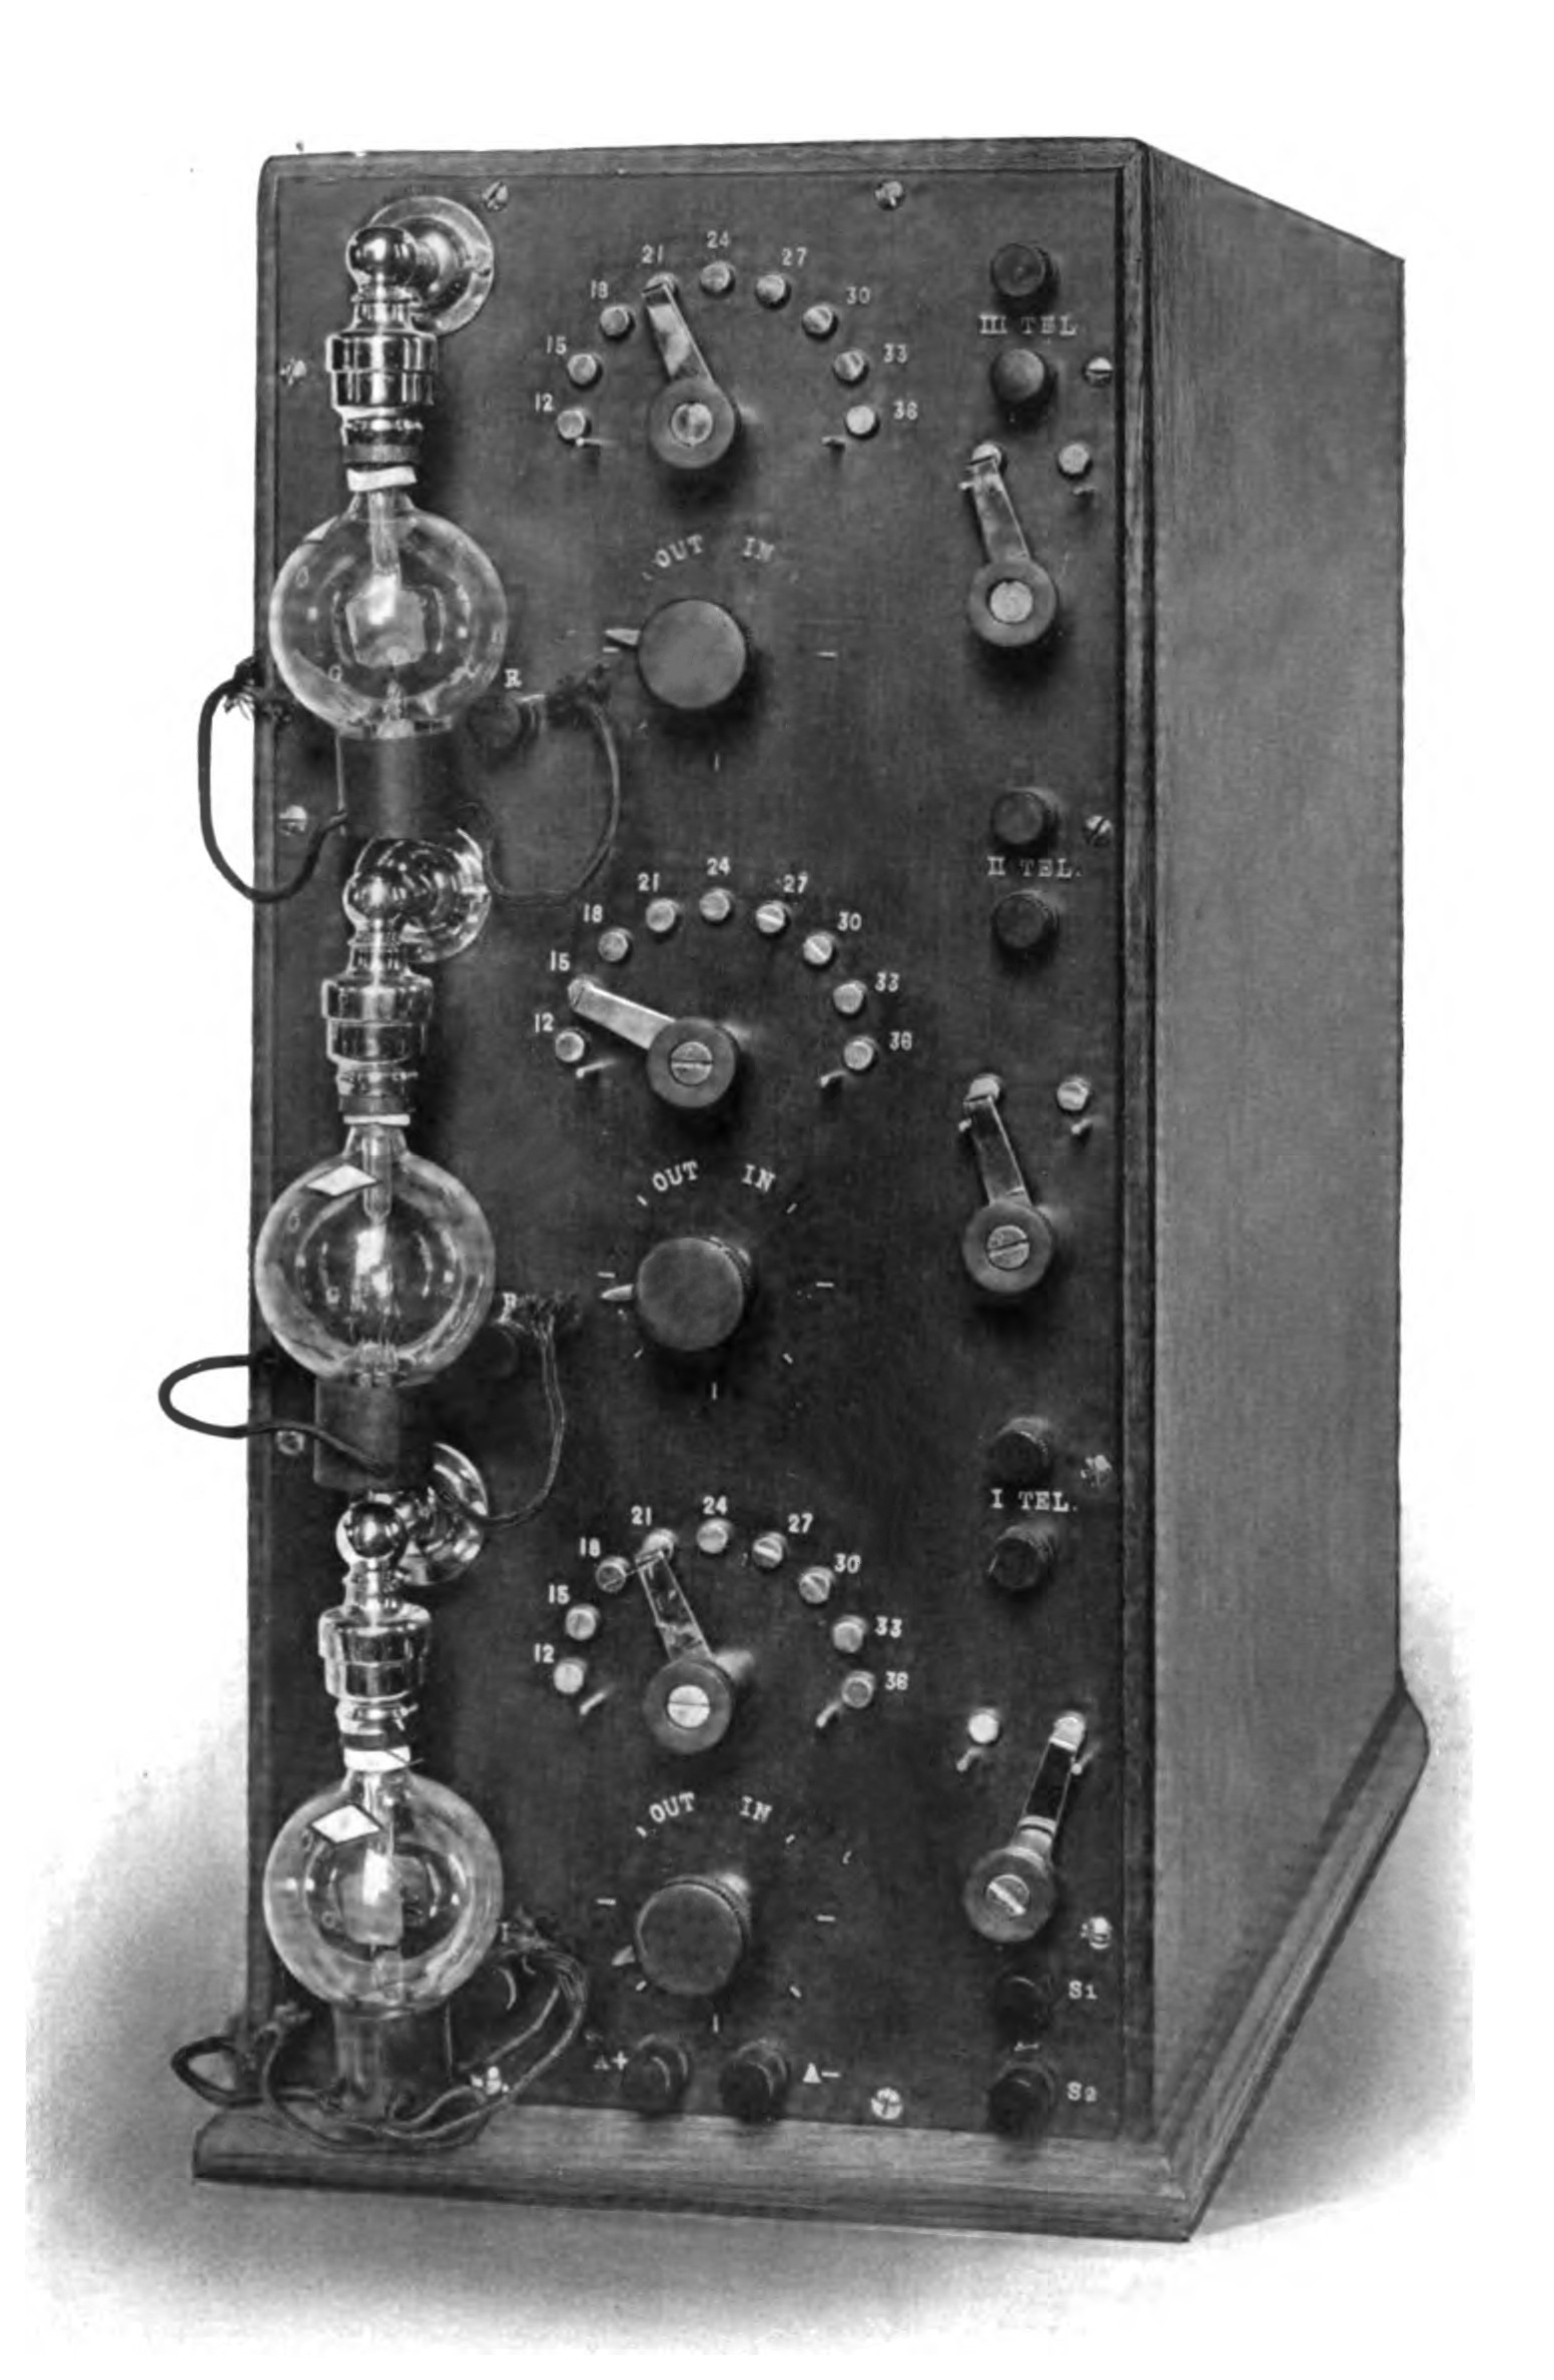
\includegraphics[scale = 0.1]{Figures/First_Audion_amplifier_1914.jpg}
        \caption{De Forest's prototype audio amplifier of 1914. The Audion (triode) vacuum tube had a voltage gain of about 5, providing a total gain of approximately 125 for this three-stage amplifier.}
        \label{fig:prism}
    \end{figure}
    \par
    An \textbf{electronic amplifier} is an electronic device that can increase the power of a signal (a time-varying voltage or current). It is a two-port electronic circuit that uses electric power from a power supply to increase the amplitude of a signal applied to its input terminals, producing a proportionally greater amplitude signal at its output. The amount of amplification provided by an amplifier is measured by its gain: the ratio of output voltage, current, or power to input. An amplifier is a circuit that has a power gain greater than one. We have already dealt with different types of amplifiers constructed using transistors such as the \textit{operational amplifier} (op amps) which is a DC-coupled high-gain electronic voltage amplifier with a differential input and, usually, a single-ended output and its subsequent applications.
    \par
    In this experiment, our focus will be on the \textbf{Lock-in amplifier}, which is a type of amplifier that can extract a signal with a known carrier wave from an extremely noisy environment. Depending on the dynamic reserve of the instrument, signals up to 1 million times smaller than noise components, potentially fairly close by in frequency, can still be reliably detected. The lock-in amplifier is capable of measuring very small AC voltages in the presence of noise. It is essentially a homodyne \footnote{a method of extracting information encoded as modulation of the phase and/or frequency of an oscillating signal, by comparing that signal with a standard oscillation that would be identical to the signal if it carried null information.} detector followed by low-pass filter that is often adjustable in cut-off frequency and filter order. Whereas traditional lock-in amplifiers use analog frequency mixers and RC filters for the demodulation, state-of-the-art instruments have both steps implemented by fast digital signal processing, for example, on an FPGA \footnote{field-programmable gate array, an integrated circuit designed to be configured by a designer after manufacturing.}.
    \par
    The lock-in amplifier uses the principle of \textit{phase sensitive detection}. It produces a maximum DC output when the signal to be measured is in phase with a reference signal at the same frequency. The lock-in amplifier employed in the experiment can work in the frequency range $\SI{100}{\hertz}$ to $\SI{5}{\kilo \hertz}$. An AC signal of $\SI{200}{\micro \volt}$ \textit{root mean square} amplitude will produce a DC output of about $\SI{1}{\volt}$. 
    \par
    \begin{figure}
        \centering
        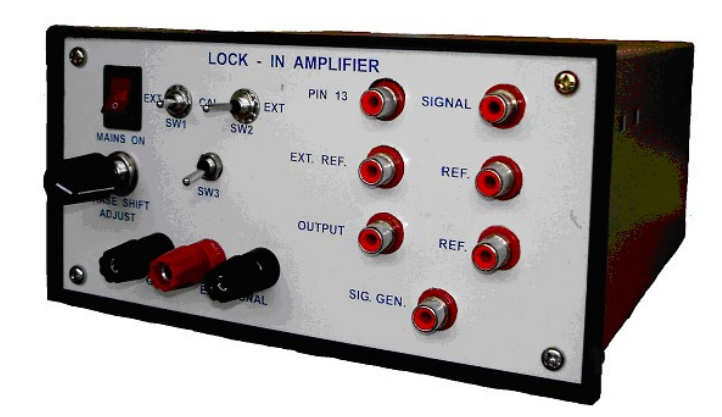
\includegraphics[scale = 0.5]{Figures/lockin.png}
        \caption{Lock-in Amplifier used in the experiment}
        \label{fig:lockin}
    \end{figure}
    \par
    The lock-in amplifier is commonly believed to have been invented by Princeton University physicist Robert H. Dicke although he claims that he read about it in a review of scientific equipment written by Walter C. Michels, a professor at Bryn Mawr College along with Norma L. Curtis in 1941.
    
\section{\label{sec:setup}Description of the Setup}
    The mains switch is at the top left hand corner of the front panel. When the switch is pressed down the lock-in amplifier is powered and an indicator light in the switch comes on. On the right half of the front panel there are a number of $RCA$ sockets which carry the audio signal. A signal generator is connected to this socket for internal calibration of the lock-in amplifier. The calibration process in itself is part of the experiment and will be detailed later. Above the sig-gen (signal generator) $RCA$ socket, we have two other sockets marked $REF$ and $REF'$. These are sockets which can be connected to a two-channel oscilloscope to display the reference signal and the phase shifted reference signal respectively.
    \par
    The reference signal is phase shifted by turning the knob of a pot marked \textit{phase shift adjust}. The $RCA$ socket marked \textit{signal} can be connected to an oscilloscope to show the amplified small AC signal with noise. The RCA socket marked \textit{pin 13} shows the output of the chip $AD630$. The $AD630$ is a high precision balanced modulator which combines a flexible commutating architecture with the accuracy and temperature stability afforded by laser wafer trimmed thin-film resistors. Its signal processing applications include balanced modulation and demodulation, synchronous detection, phase detection, quadrature detection, phase sensitive detection, lock-in amplification and square wave multiplication. It may be thought of as a precision op amp with two independent differential input stages and a precision comparator which is used to select the active front end.
    \par
    As the phase shift adjust knob is turned the pattern of the output at pin 13, as seen on an oscilloscope, changes. When the phase-shifted reference is in phase with the signal, the output at pin 13 looks like the output of a full wave rectifier. The RCA pin marked \textit{output} is connected to a digital multimeter in an appropriate $DC$ range. This measures the amplified $DC$ output from pin 13 of the lock-in chip. 
 
    \begin{figure*}
        \centering
        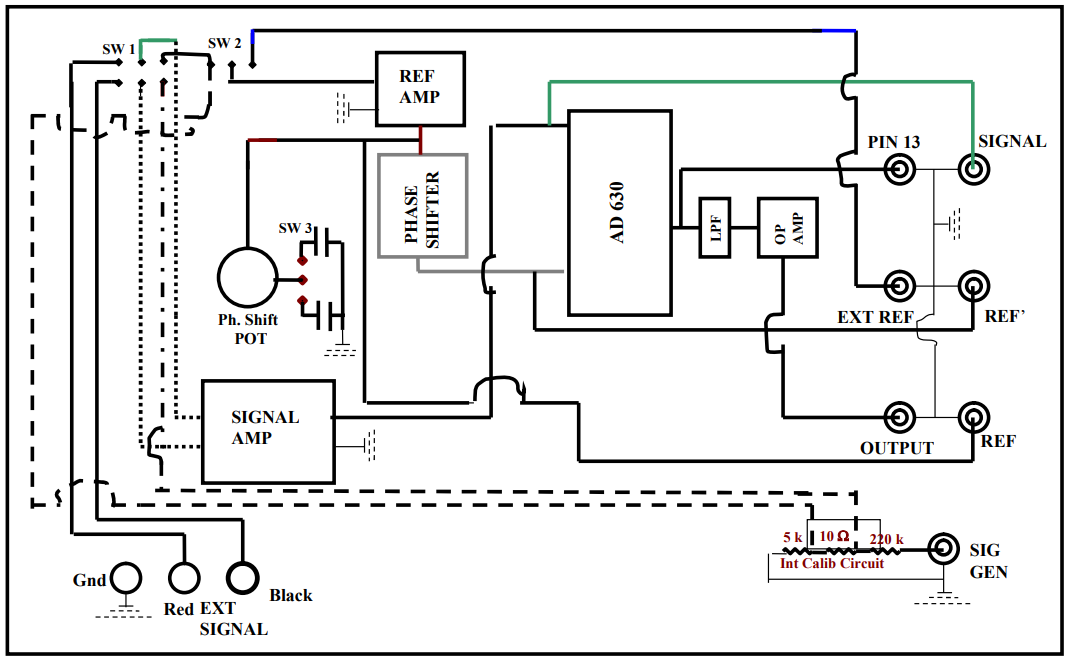
\includegraphics[scale = 0.75]{Figures/schematic.png}
        \caption{Schematic diagram of the lock-in amplifier circuit}
        \label{fig:schematic}
    \end{figure*}
    \par
    There are two toggle switches. When both are put in $CAL$ mode one can  internally calibrate the lock-in as explained later in section \ref{sec:calib}. When an external signal is to be measured the toggle switches are put in position $EXT$. In this mode, the external $AC$ signal should be connected to the two banana terminals (red and black) at the bottom of the front panel. The external reference signal should be connected to the $RCA$ socket marked $EXT$ $REF$.
    \par
    In the schematic diagram of the lock-in amplifier circuit in figure (\ref{fig:schematic}), all the front panel controls are marked. The internal calibration circuit consists of three resistances, $\SI{220}{\kilo \ohm}$, $\SI{10}{\ohm}$ and $\SI{5}{\kilo \ohm}$ in series across which the $AC$ voltage from the signal generator is applied. The voltage across $\SI{10}{\ohm}$ provides the internally generated signal used for calibration. The voltage across the $\SI{5}{\kilo \ohm}$ provides the internally generated reference signal. When the switch $SW 1$ is put in the position $CAL$ the internally generated signal is connected to the signal amplifier. Similarly when the switch $SW2$ is put to the position marked $CAL$ the internally generated reference signal is connected to the reference amplifier.
    \par
    When measurements on external systems have to be done, the switches $SW1$ and $SW2$ are put in the positions marked $EXT$. The signal generated from the external circuit is connected to the red and black banana terminals marked $EXT$ $SIGNAL$. Similarly the reference signal from the external circuit is connected to the $RCA$ socket marked $EXT$ $REF$. When the switches $SW1$ and $SW2$ are in the external position the external signal is connected to the signal amplifier and the external reference to the reference amplifier. The signal coming out of the signal amplifier is fed to pin 1 of $AD630$ chip.
    \par
    The reference signal after amplification goes to a phase shifter. Phase shifting is achieved by an $RC$ network. $R$ is a pot which can be adjusted by turning a knob marked phase shift. The maximum phase shift that one can achieve is given by the product of frequency $f$, $C$ and $R$. At frequencies below $\SI{1}{\kilo \hertz}$, one has to use a larger capacitance to achieve a phase shift close to $\SI{180}{\degree}$ at the maximum resistance in the pot. At frequencies greater than $\SI{1}{\kilo \hertz}$, the use of the same capacitor will cause the phase to be shifted rapidly as the resistance in the pot is increased. To make the phase change more gradual in the frequency range $\SI{1}{\kilo \hertz}$ to $\SI{10}{\kilo \hertz}$, a smaller capacitance is used. The switch SW3 selects the capacitor. At frequencies below $\SI{1}{\kilo \hertz}$ the switch is put in the up position and at frequencies greater than $\SI{1}{\kilo \hertz}$ the switch is put in the down position.
    \par
    The reference signal after phase shifting is connected to pin 9 of the $AD630$ chip. Leads are taken from the input of the phase shifter and from pin 9 of $AD630$ to two $RCA$ sockets marked $REF$ and $REF'$ respectively. By connecting $REF$ and $REF'$ to two channels of an oscilloscope one can see how much the phase is shifted on turning the pot. When the signal to be measured and the phase shifted reference signal match in phase the output at pin 13 of $AD630$ looks like that of a full wave rectifier. A lead is taken from pin 13 to an $RCA$ socket marked \textit{pin 13} on the front panel. By connecting it to an oscilloscope one may see how the output at pin 13 varies as the phase of the reference signal is shifted. This output of $AD630$ is connected to a low pass filter (LPF) and then to an output amplifier. The output of this amplifier is connected to an $RCA$ socket marked OUTPUT. A digital multimeter in the appropriate voltage range connected to this socket measures the $DC$ output of the lock in amplifier.
    \par
    A lead is taken to an $RCA$ socket marked signal on the front panel. By connecting it to an oscilloscope one can see the trace of the signal. At frequencies greater than about $\SI{1}{\kilo \hertz}$ there is a distortion in the reference signal as seen at $REF$ and $REF'$, but for our experiment we will be ignoring its effects, if any. 

\section{Theory}
    Before using the amplifier, we must understand that the process also amplifies the noise. Amplifiers operate over a bandwidth spanning several kilohertz, and while the noise is present over a range of several frequencies, the signal is at a single frequency.
    \par
    There are various sources of noise in an amplifier. Flicker noise is present in all electronic instruments and its power spectrum varies inversely with the frequency. Then we have noise due to electromagnetic radiation pick up from running motors, tube lights and so on. This type of noise can be reduced by electromagnetic shielding. Lastly, there is thermal noise which cannot be avoided.
    \par
    If we have resistance $R$ through which a current $I$ is flowing the voltage across the resistance will vary randomly about the average value $V_0 = IR$. The mean square fluctuation of the voltage is defined by $< (V-V_0)^2 >$ where the average is taken over a long period of time. If we measure the noise over a bandwidth $W$, the mean square voltage will be
    \begin{equation}
        < (V-V_0)^2 > = 4 k_B T_K R W
    \end{equation}
    $T_K$, being the temperature. We can reduce this noise by reducing $T_K$ or the bandwidth of the amplifier $W$. The latter at room temperature is achieved by \textit{phase sensitive detection}.
    \par
    Let us have an AC sinusoidal cause. If we merely amplify the weak signal a million times we will also amplify the noise. In an ordinary amplifier the noise is collected over a wide frequency range and so may even swamp the weak signal due to the cause.
    \par
    To overcome the noise vis-à-vis the weak effect signal, we take a reference signal, which is derived from the cause signal and is in phase with it. The weak effect signal and the reference signals are presented in the figures (\ref{fig:weaksig}) and (\ref{fig:refvol}) respectively.
    \begin{figure}
        \centering
        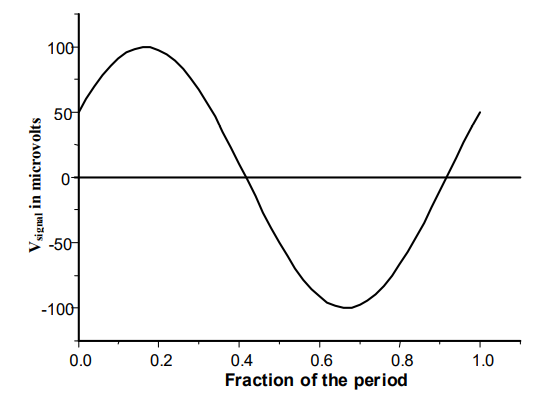
\includegraphics[scale = 0.69]{Figures/weaksignal.png}
        \caption{Weak signal as a function of time ($t/T$) where $T$ is the period.}
        \label{fig:weaksig}
    \end{figure}
    \begin{figure}
        \centering
        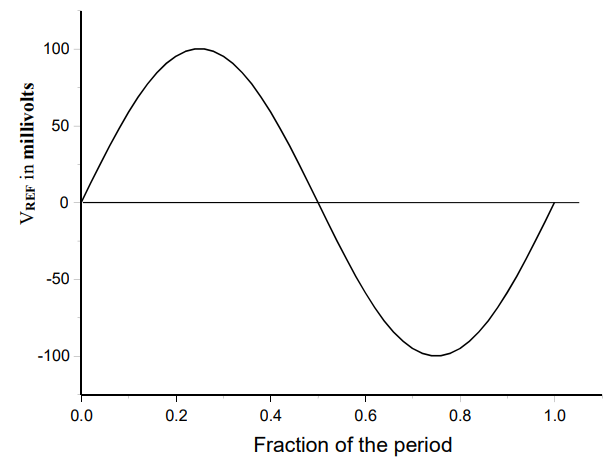
\includegraphics[scale = 0.6]{Figures/refvoltage.png}
        \caption{Reference voltage as a function of time ($t/T$) where $T$ is the period.}
        \label{fig:refvol}
    \end{figure}
    From the above figures it is seen that the weak signal is advanced in phase relative to reference signal by an angle $\phi$. In the above example $\phi = \pi/6$.
    \par
    We may write
    \begin{equation}
        V_{sig} = V_0 \sin (\omega t + \phi)
    \end{equation}
    and
    \begin{equation}
        V_{ref} = V_0 \sin (\omega t)
    \end{equation}
    Assume that these are the magnitudes of the signal and reference voltage after some amplification in our circuit. These signals are then fed to the chip $AD630$. This is a \textit{phase sensitive detector}. In this chip there are two identical amplifiers. One is a direct amplifier,whose output is in phase with the input. The other is an inverse amplifier whose output is $180 \degree$ out of phase with the input. There is a switch operated by a comparator. The comparator senses the reference signal. When the reference signal is positive (that is, for $0 < t < T/2$), the comparator connects the weak signal $V_{sig}$ to the direct amplifier so that the output of the amplifier is
    \begin{equation}
        V_{out} = \mu V_{sig} \hspace{1cm} (0 < t < T/2)
    \end{equation}
    $\mu$ being the amplification factor or voltage gain of the $AD630$. When the reference signal is negative (that is, for $T/2 < 0 < T$) the weak signal is connected to the inverse amplifier so that the output voltage is
    \begin{equation}
        V_{out} = - \mu V_{sig} \hspace{1cm} (T/2 < t < T)
    \end{equation}
    \begin{figure}
        \centering
        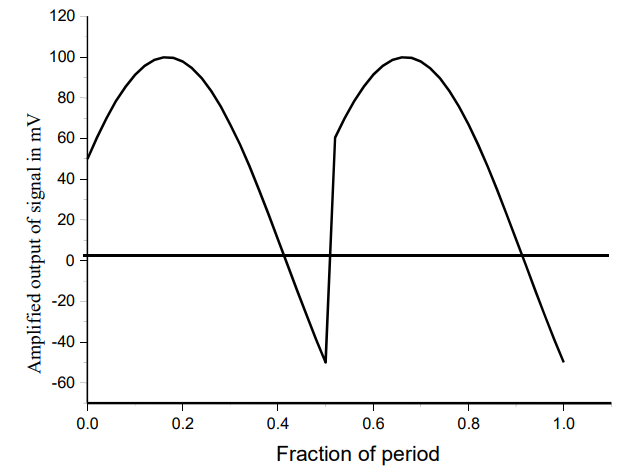
\includegraphics[scale = 0.6]{Figures/ampoutputComp.png}
        \caption{Amplified output signal $V_{out}$ when the reference signal is fed to the comparator.}
        \label{fig:outcomp}
    \end{figure}
    Figure (\ref{fig:outcomp}) shows the amplified signal $V_{out}$ assuming an amplification of 1000. We observe that the output signal is positive for most of the period but there is a small negative portion. So the output signal will have an average DC part superposed on an AC part at the frequencies $\omega, 2 \omega, \ldots$. We calculate the $DC$ output from the equation
    \begin{equation}
        \begin{split}
            V_{DC}
            &= \dfrac{1}{T} \Bigg( \int_{0}^{T/2} \mu V_0 \sin (\omega t + \phi) dt \\ 
            &- \int_{T/2}^{T} \mu V_0 \sin (\omega t + \phi) dt \Bigg) \\
            &= \dfrac{4 \mu V_0}{2 \pi} \cos (\phi)
        \end{split}
    \end{equation}
    remembering $\omega T = 2 \pi$.
    \par
    If we introduce a circuit to phase shift the reference signal and then send the phase shifted reference signal to the comparator in $AD630$, the output $DC$ voltage will vary as the phase shift is increased from zero. It will reach a maximum when the reference signal is phase shifted by $\phi$ and the phase-shifted reference signal is in phase with the weak signal $V_{sig}$. Then the output voltage will look like the one shown in figure (\ref{fig:outad630}). The average $DC$ voltage, $V_{DC}$, will then reach a maximum value $2 \mu V_0 / \pi$.
    \begin{figure}
        \centering
        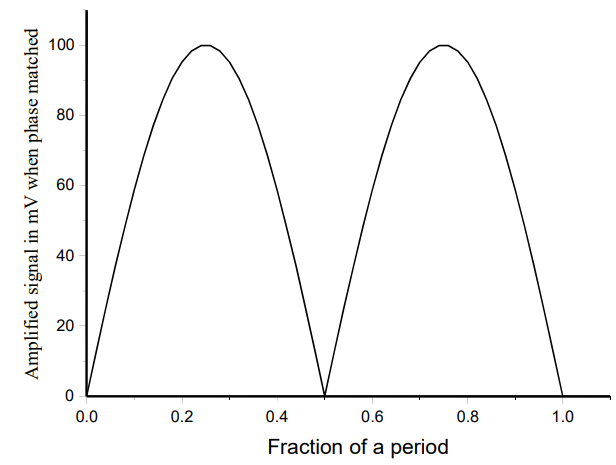
\includegraphics[scale = 0.6]{Figures/ampoutputAD630.png}
        \caption{Amplified output signal when the reference signal is phase shifted by $\phi$ and fed to $AD630$ chip}
        \label{fig:outad630}
    \end{figure}
    \par
    As we make the weak signal lock in phase with the phase-shifted reference to give maximum DC output voltage, this method is called phase sensitive detection, and the amplifier as a \textit{lock-in} amplifier.
    \par
    From this discussion, we can show that the contribution of the noise with frequency $\omega'$ to $V_{DC}$ drops rapidly as $\omega'$ differs from reference signal frequency $\omega$. If $\tau$, the integration time is large compared to the period of the reference signal, then only noise frequencies differing from $\omega$ by $n/\tau$ (where n is a small number) will make a contribution to $V_{DC}$. This means that the effective bandwidth of the lock-in amplifier is  $n/\tau$. It can be thus understood, that how thermal and other noises are suppressed by the lock-in amplifier.
    
\section{\label{sec:calib}Calibration}
    Before using the lock-in amplifier for experiments, one must calibrate it. Calibration means measuring the maximum output $DC$ voltage of the lock-in amplifier for a small known $AC$ signal voltage as a function of the frequency of the signal.
    \par
    The apparatus required for this purpose is a signal generator, a lock-in amplifier, two channel oscilloscope and a digital multimeter to measure $DC$ volts to three decimal places in the $\SI{2}{\volt}$ range. 
    \subsubsection{Experimental Procedure}
    \begin{enumerate}
        \item We connect a signal generator (described in Section \ref{sec:setup}) to the $RCA$ socket marked $SIG$ $GEN$ at the bottom of the front panel of the lock-in amplifier (LIA).
        \item The switches SW1 and SW2 are then thrown to the position marked $CAL$ and the internal calibration circuit is connected to the LIA chip.
        \item The frequency of the signal generator is set at 500 HZ. The amplitude ($V_{app}$) of the signal generator is adjusted at about $\SI{4}{\volt}$.
        \item Inside the LIA, voltage is applied to the three resistances ($\SI{220}{\kilo \ohm}$, $\SI{10}{\ohm}$ and $\SI{5}{\kilo \ohm}$). The voltage across the $\SI{10}{\ohm}$ resistor is given by
            \begin{equation}
            \label{eq7}
                V_{sig} = V_{app} \times \dfrac{10 \ohm}{(220 + 5) \ohm} = 44.4 V_{app} \mu V
            \end{equation}
        \item The switch $SW3$ is turned up and the phase shifter potentiometer knob is turned to the right extreme (resistance and phase shift both being zero).
        \item The $RCA$ sockets marked $REF$ and $REF'$ are connected to the two channels of an oscilloscope. Two amplified reference signals in form of sinusoidal traces appear at the frequency of the signal generator, one before phase shifting and the other after phase shifting. Since the phase shift is zero when the phase adjusting pot is at the extreme right, the two traces will be superposed exactly indicating zero phase shift.
        \item The $DC$ voltage is noted using the digital multimeter on the $\SI{2}{\volt}$ range.
        \item The phase shifter potentiometer knob is turned and adjusted so that the $DC$ voltage on the multimeter is zero. This makes the maxima of the $REF'$ signal now occur at the position of zeroes of the $REF$ signal, indicating a phase shift of $90 \degree$. If the knob is turned further, the phase shift increases beyond $90 \degree$, the panel meter reading becomes negative. When the knob of the potentiometer is to the left end, the phase shift is nearly (but less than) $180 \degree$ and the panel meter indicates the negative largest value. In the calibration circuit, the signal and reference voltages are derived from the potential differences across two resistances in series. They are in phase. So the panel meter voltage is largest when the phase shift is zero.
        \item The $RCA$ socket marked \textit{pin 13} is connected to the oscilloscope and the changes in output of the LIA are observed.
        \item The knob of the potentiometer is turned to the extreme right and the corresponding steady $DC$ voltage value, $V_{DC}$ on the multimeter is noted. This is repeated for multiple values of the output of the signal generator from $\SI{1.5}{\volt}$ to $\SI{4}{\volt}$ in steps of $\SI{0.5}{\volt}$, keeping the frequency fixed.
        \item $V_{sig}$ is calculated from equation (\ref{eq7}) and plotted against $V_{DC}$. The slope, $\mu$, thus found is the amplification factor of the corresponding frequency. The whole process is performed multiple times for different frequencies.
    \end{enumerate}
    \subsubsection{Observations}
    The readings obtained from the procedure for various frequencies are tabulated in table (\ref{tab:calib}). In converting $V_{AC}$ into $V_{sig}$ we use the conversion factor as given in equation (\ref{eq7}) for one volt from the signal generator. The plots are plotted in figure (\ref{fig:calibdata}).
    \par
    The amplification factor $\mu$ so obtained is tabulated against different frequencies with corresponding standard deviations in table (\ref{tab:calibamp}). Note that the amplification factor can vary from a lock-in amplifier to another lock-in amplifier.
    \begin{table*}[]
    \caption{\label{tab:calib} Readings for the calibration of the lock-in amplifier}
    \centering
    \resizebox{\textwidth}{!}{%
    \begin{tabular}{ccccccccccccccccccccccccccccccccc} \\ \toprule
    \multicolumn{3}{c}{$f = \SI{500}{\hertz}$} & \phantom{abc} & \multicolumn{3}{c}{$f = \SI{1000}{\hertz}$} & \phantom{abc} & \multicolumn{3}{c}{$f = \SI{1500}{\hertz}$} & \phantom{abc} & \multicolumn{3}{c}{$f = \SI{2000}{\hertz}$} & \phantom{abc} & \multicolumn{3}{c}{$f = \SI{2500}{\hertz}$} & \phantom{abc} & \multicolumn{3}{c}{$f = \SI{3000}{\hertz}$} \\ \midrule
    \begin{tabular}[c]{@{}c@{}}$V_{AC}$\\ \scriptsize (V) \end{tabular} & \begin{tabular}[c]{@{}c@{}}$V_{sig}$\\ \scriptsize ($\mu$ V)\end{tabular} & \begin{tabular}[c]{@{}c@{}}$V_{DC}$\\ \scriptsize (V)\end{tabular} && \begin{tabular}[c]{@{}c@{}}$V_{AC}$\\ \scriptsize (V)\end{tabular} & \begin{tabular}[c]{@{}c@{}}$V_{sig}$\\ \scriptsize ($\mu$ V)\end{tabular} & \begin{tabular}[c]{@{}c@{}}$V_{DC}$\\ \scriptsize (V)\end{tabular} && \begin{tabular}[c]{@{}c@{}}$V_{AC}$\\ \scriptsize (V)\end{tabular} & \begin{tabular}[c]{@{}c@{}}$V_{sig}$\\ \scriptsize ($\mu$ V)\end{tabular} & \begin{tabular}[c]{@{}c@{}}$V_{DC}$\\ \scriptsize (V)\end{tabular} && \begin{tabular}[c]{@{}c@{}}$V_{AC}$\\ \scriptsize (V)\end{tabular} & \begin{tabular}[c]{@{}c@{}}$V_{sig}$\\ \scriptsize ($\mu$ V)\end{tabular} & \begin{tabular}[c]{@{}c@{}}$V_{DC}$\\ \scriptsize (V)\end{tabular} && \begin{tabular}[c]{@{}c@{}}$V_{AC}$\\ \scriptsize (V)\end{tabular} & \begin{tabular}[c]{@{}c@{}}$V_{sig}$\\ \scriptsize ($\mu$ V)\end{tabular} & \begin{tabular}[c]{@{}c@{}}$V_{DC}$\\ \scriptsize (V)\end{tabular} && \begin{tabular}[c]{@{}c@{}}$V_{AC}$\\ \scriptsize (V)\end{tabular} & \begin{tabular}[c]{@{}c@{}}$V_{sig}$\\ \scriptsize ($\mu$ V)\end{tabular} & \begin{tabular}[c]{@{}c@{}}$V_{DC}$\\ \scriptsize (V)\end{tabular} \\ \midrule
    1.65 & 73.33 & 0.116 && 
    1.65 & 73.33 & 0.113 && 
    1.65 & 73.33 & 0.125 &&
    1.65 & 73.33 & 0.129 && 
    1.65 & 73.33 & 0.129 && 
    1.65 & 73.33 & 0.132 \\
    2 & 88.89 & 0.14 && 
    2 & 88.89 & 0.143 && 
    2 & 88.89 & 0.152 && 
    2 & 88.89 & 0.158 && 
    2 & 88.89 & 0.158 && 
    2 & 88.89 & 0.159 \\
    2.5 & 111.11 & 0.17 && 
    2.5 & 111.11 & 0.178 && 
    2.5 & 111.11 & 0.177 && 
    2.5 & 111.11 & 0.18 && 
    2.5 & 111.11 & 0.192 && 
    2.5 & 111.11 & 0.198 \\
    3 & 133.33 & 0.208 && 
    3 & 133.33 & 0.209 && 
    3 & 133.33 & 0.216 && 
    3 & 133.33 & 0.219 && 
    3 & 133.33 & 0.221 && 
    3 & 133.33 & 0.224 \\
    3.5 & 155.56 & 0.24 && 
    3.5 & 155.56 & 0.243 && 
    3.5 & 155.56 & 0.25 &&
    3.5 & 155.56 & 0.26 && 
    3.5 & 155.56 & 0.263 && 
    3.5 & 155.56 & 0.26 \\
    4 & 177.78 & 0.269 && 
    4 & 177.78 & 0.275 && 
    4 & 177.78 & 0.282 && 
    4 & 177.78 & 0.287 && 
    4 & 177.78 & 0.293 && 
    4 & 177.78 & 0.3 \\ \bottomrule
    \end{tabular}%
    }
    \end{table*}
    \begin{figure}
        \centering
        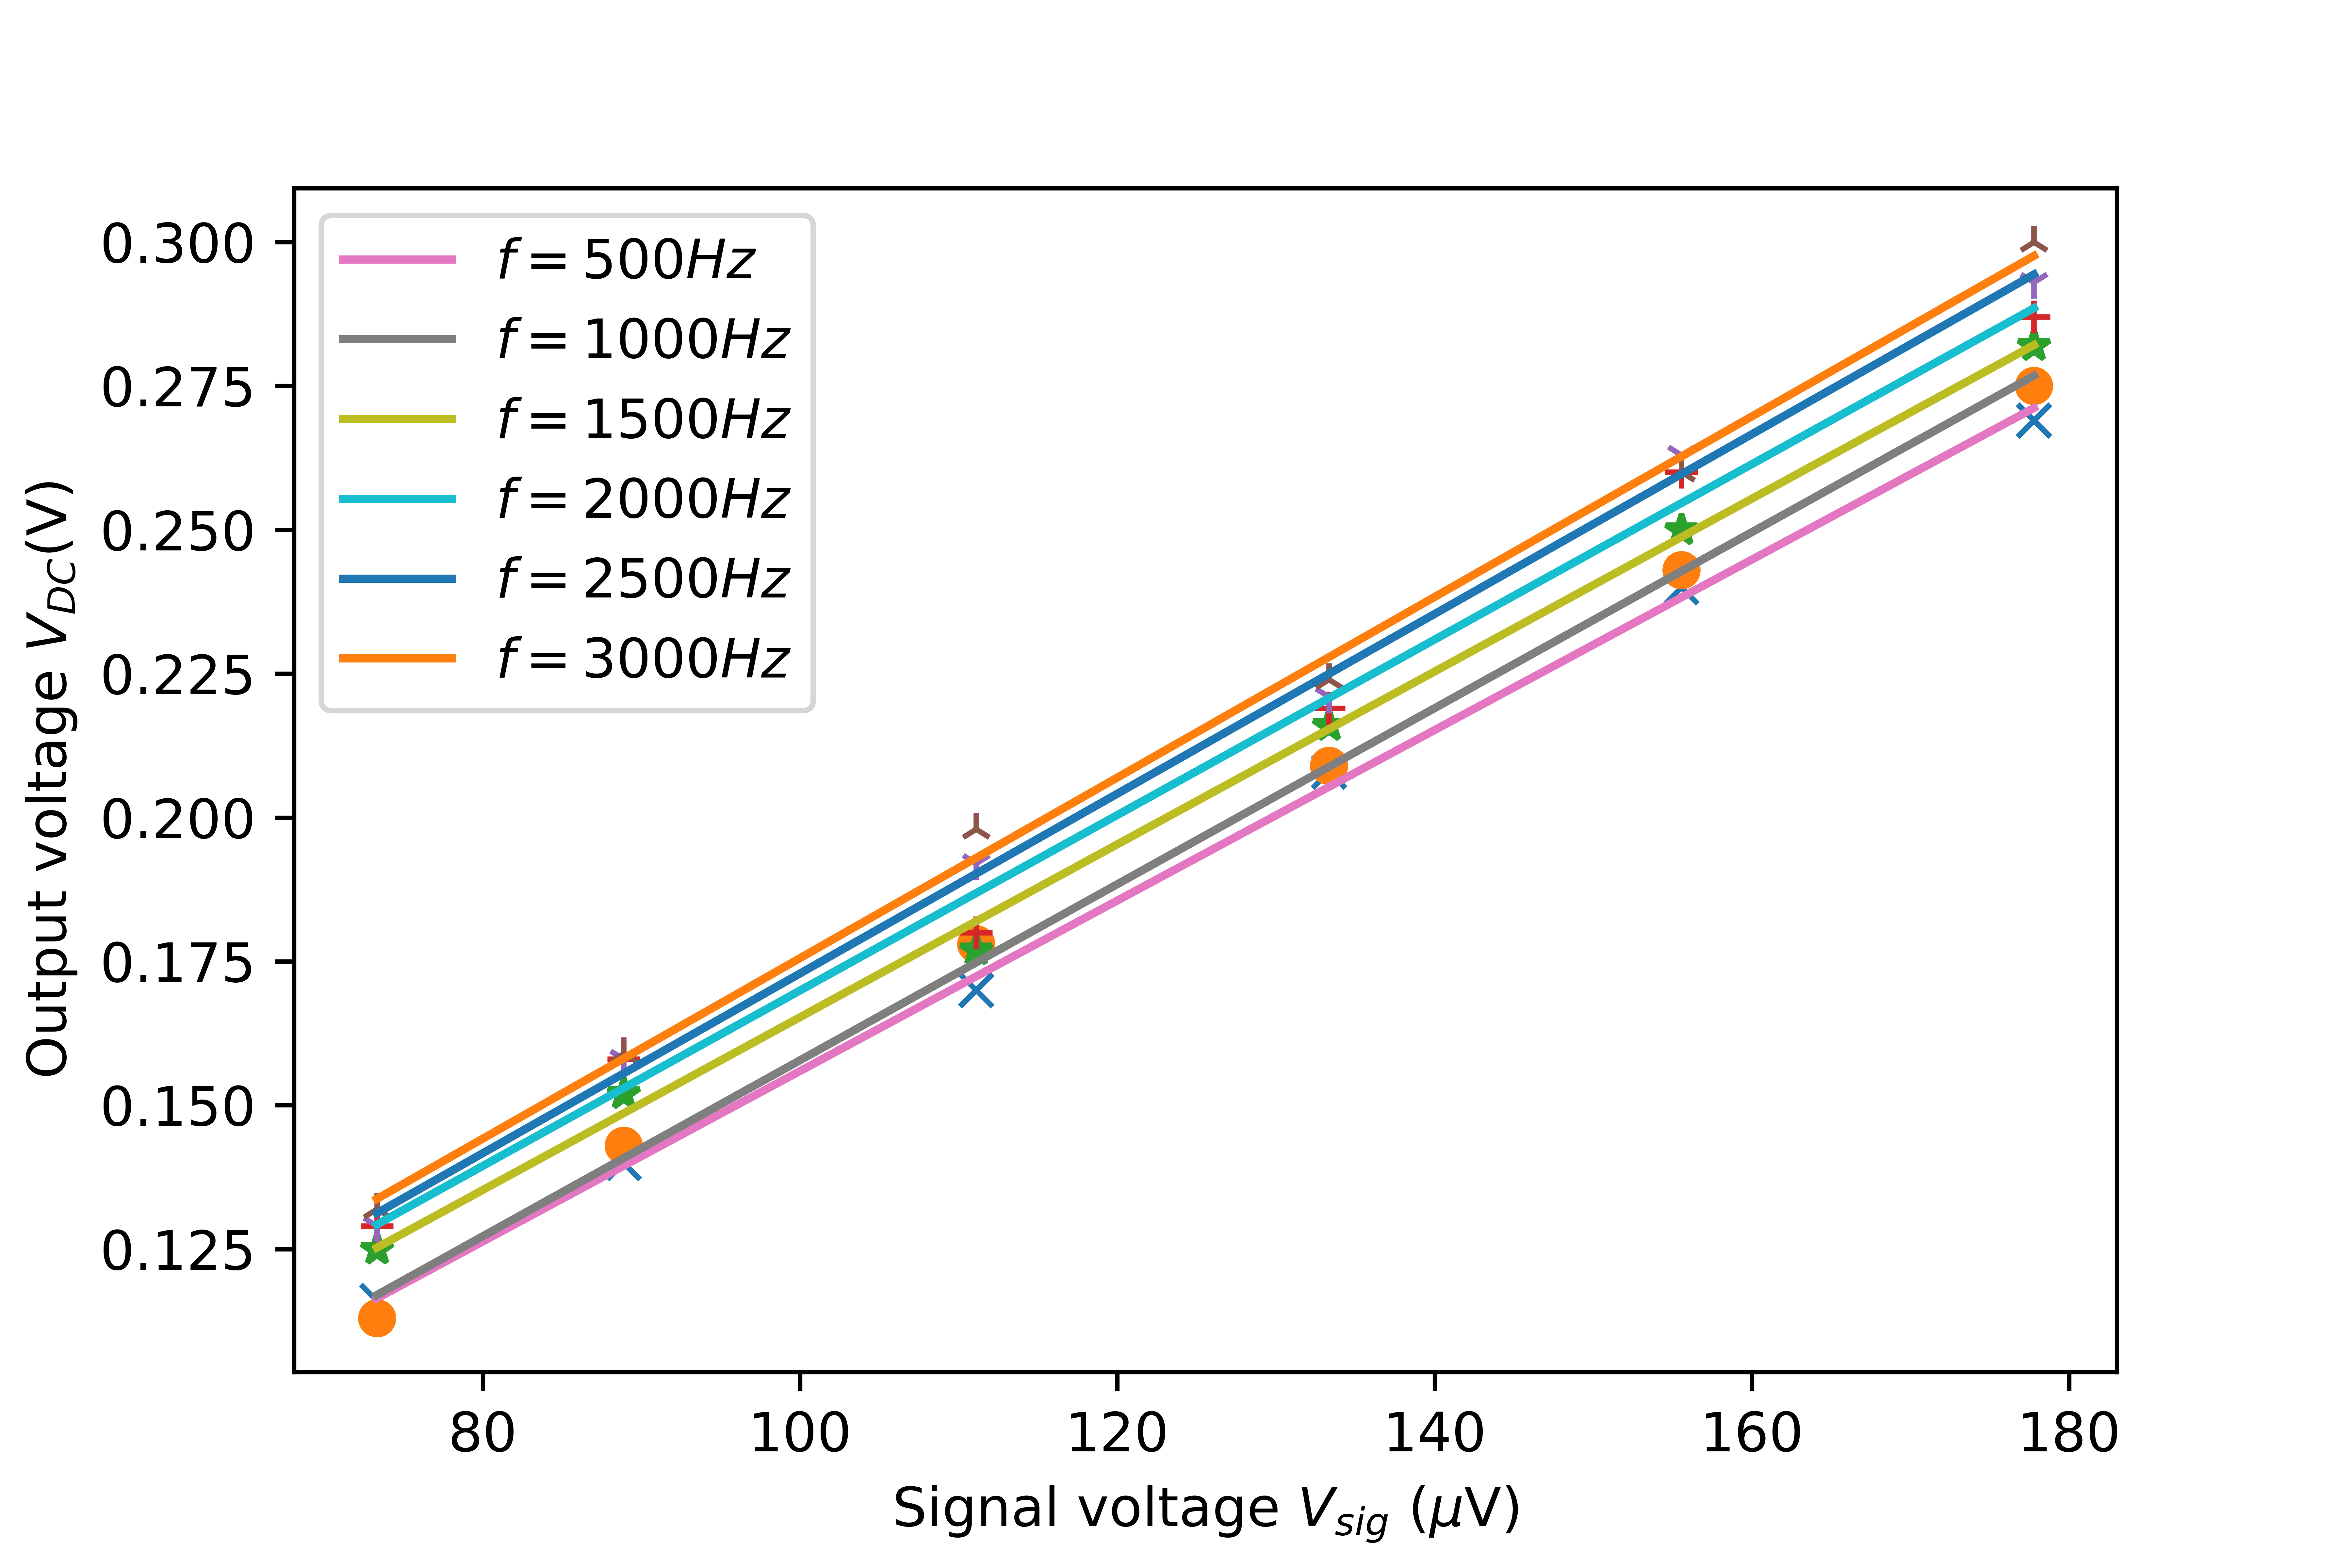
\includegraphics[scale = 0.56]{Figures/plot-calib.png}
        \caption{$V_{DC}$ in volts against $V_{sig}$ in microvolts for various frequencies}
        \label{fig:calibdata}
    \end{figure}
    \begin{table}[]
    \caption{\label{tab:calibamp}Amplification factor $\mu$ at different frequencies}
    \centering
    \begin{tabular}{ccc}
    \toprule
    \begin{tabular}[c]{@{}c@{}}Frequency $f$\\ (kHz)\end{tabular} & \begin{tabular}[c]{@{}c@{}}Amplification factor $\mu$\\ ($\times 10^3$)\end{tabular} & \begin{tabular}[c]{@{}c@{}}Deviation\\ ($\times 10^3$)\end{tabular} \\
    \midrule
    0.5 & 1.48 & 0.026 \\
    1   & 1.53 & 0.033 \\
    1.5 & 1.50 & 0.035 \\
    2   & 1.52 & 0.058 \\
    2.5 & 1.56 & 0.037 \\
    3   & 1.57 & 0.042 \\
    \bottomrule
    \end{tabular}
    \end{table}
    
    
    
\section{Experiments}
    After the calibration procedure is completed, we can move on to performing experiments with the lock-in amplifier. We will be using the lock-in amplifier with mutual inductance coil and low-resistance boxes and will draw various conclusions which can corroborate our understanding about the lock-in amplifier.
    
    \subsection{With a mutual inductance coil}
        Inductance is the tendency of an electrical conductor to oppose a change in the electric current flowing through it. The flow of electric current creates a magnetic field around the conductor. The field strength depends on the magnitude of the current, and follows any changes in current. From Faraday's law of induction, any change in magnetic field through a circuit induces an \textit{electromotive force} (EMF) (voltage) in the conductors, a process known as \textit{electromagnetic induction}. This induced voltage created by the changing current has the effect of opposing the change in current.
        \par
        When two coils are placed side by side and an $AC$ current is passed through one coil (called the primary), an $AC$ voltage at the same frequency is induced in the other coil (called the secondary) (see figure (\ref{fig:mutintro})). \textit{Mutual inductance} is defined as the ratio between the emf induced in one loop or coil by the rate of change of current in another loop or coil. Mutual inductance is given the symbol $M$.
        \begin{figure}
            \centering
            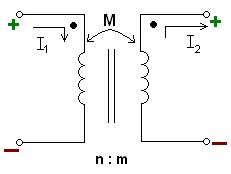
\includegraphics{Figures/Mutually_inducting_inductors.png}
            \caption{Circuit diagram of two mutually coupled inductors}
            \label{fig:mutintro}
        \end{figure}
        \par
        If primary current varies as
        \begin{equation}
            I = I_0 \sin (2 \pi f t)
        \end{equation}
        where $f$ is the frequency in hertz, the emf induced in the secondary is
        \begin{equation}
        \label{eq9}
            \begin{split}
                V
                &= - M \dfrac{dI}{dt} \\
                &= -2 \pi M f I_0 \cos (2 \pi f t) \\
                &= -2 \pi M f I_0 \sin (2 \pi f t + \pi/2)
            \end{split}
        \end{equation}
        Hence, we note that
        \begin{enumerate}
            \item The phase difference between the primary current and the induced emf is $\pi/2$.
            \item The secondary emf is proportional to the amplitude $I_0$ of the primary current.
            \item The induced emf is proportional to the frequency $f$.
        \end{enumerate}
        Through our experiment with the lock-in amplifier, we will be verifying all these results.
        \par
        The appratus required for this experiment is a signal generator, a lock-in amplifier, a two-channel oscilloscope, a mutual inductance coil, one digital multimeter to measure $AC$ frequency exactly, and one digital multimeter to measure $DC$ output of lock-in amplifier to two decimal places in $DC$ $\SI{20}{\volt}$ range. 

        \subsubsection{The Mutual Inductance coil}
            On an insulating former a coil of about 20 turns is wound using insulated copper wire (see figure (\ref{fig:mutinductcoil})), which can carry a current of about a few milli-ampere. There are three banana terminals red, yellow and black at primary end of the coil. A $\SI{4.7}{\kilo \ohm}$ resistor and the primary coil are connected between red and yellow banana terminals. Between the yellow and black a hundred ohm resistor is connected. When a signal generator is connected between the red and black terminals and an rms $AC$ voltage of $V_{rms}$ volts is applied, an rms current of
            \begin{equation}
                I_{rms} = \dfrac{V_{rms}}{R_{total}} = \dfrac{V_{rms}}{4.8 \times 10^3} \text{amps}
            \end{equation}
            flows through the primary coil. The resistance of the primary coil, which is of the order of $\SI{1}{\ohm}$, can be neglected in the denominator compared to $\SI{4800}{\ohm}$ and the voltage across $\SI{100}{\ohm}$ is used as the reference signal. The signal generator ground must be connected to the black terminal on the primary side of the coil box and the other terminal of the signal generator must be connected to the red banana terminal on the primary side of the coil box.
            \begin{figure}
                \centering
                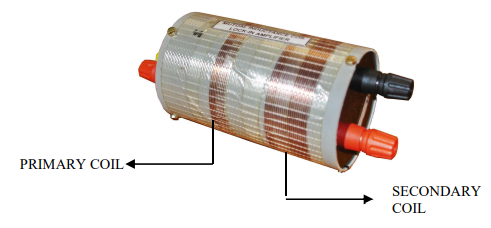
\includegraphics[scale = 0.7]{Figures/mutinductcoil.png}
                \caption{Mutual inductance coils used in the experiment}
                \label{fig:mutinductcoil}
            \end{figure}
            \par
            On the same former a second coil of about 100 turns is wound at a distance of a few centimeters from the primary coil. The terminals of the secondary coil are brought to two banana terminals on the other end of the insulating former. The emf generated by mutual inductance of the coils will appear at these terminals and will be measured by the lock-in amplifier. 
        
        
        \subsubsection{Experimental Procedure}
            As an external signal is measured here, the switches $SW1$ and $SW2$ on the LIA front panel should be set to the positions marked $EXT$.
            \begin{enumerate}
                \item The red terminal on the signal generator is connected to the red terminal and the black terminal on the signal generator to the black terminal on the primary coil side of the insulating former.
                \item The yellow and black terminals on the primary coil side of the insulating former are connected to the $RCA$ socket marked $EXT$ $REF$ on the front panel of the LIA.
                \item The red terminal on the secondary side of the insulating former is connected to the red banana terminal marked $EXT$ $SIG$ on the LIA.
                \item The black terminal on the secondary side of the insulating former is connected to the black banana terminal marked $EXT$ $SIG$ on the front panel of the LIA.
                \item A digital multimeter is connected in $DC$ $\SI{20}{\volt}$ range to the $RCA$ socket marked \textit{output} on the front panel of the LIA.
                \item The two $RCA$ sockets marked $REF$ and $REF'$ on the front panel of the LIA to the two channels of an oscilloscope.
                \item The signal generator is turned on and the amplitude on its panel meter is set to about $\SI{4}{\volt}$ and the frequency is set to about $\SI{400}{\hertz}$. The LIA and the oscilloscope are turned on and $SW3$ is put up.
                \item Two sinusoidal traces at frequency $\SI{400}{\hertz}$ appear which are in phase when the phase-shift pot on the LIA is to the extreme right. On turning the pot to left, the trace of $REF'$ shifts relative to the trace of $REF$ and the digital multimeter reading will increase (with negative sign). This process is done till a steady maximum reading is obtained. At this point, the phase difference between the two traces becomes $90 \degree$. It can be exhibited by observing the Lissajous figure (which is a distorted circle) on the oscilloscope. Further, the reference signal is in phase with the current. A maximum output of the LIA indicates that the phase-shifted reference signal is in phase with the mutual inductance emf. The Lissajous figure shows that the phase-shifted reference is $90 \degree$ out of phase with the reference signal and thus, establishing that the mutual inductance emf is $90 \degree$ out of phase with the primary current.
                \item The digital multimeter reading is noted and keeping the frequency of the signal generator the same, the amplitude is changed from $\SI{4}{\volt}$ to $\SI{1}{\volt}$ in steps of $\SI{0.5}{\volt}$.
                \item The experiment is repeated at different frequencies in steps of $\SI{200}{\hertz}$. When the frequency is $\SI{1}{\kilo \hertz}$ or more, switch $SW3$ will have to be pressed to the down position.
            \end{enumerate}
            
        \subsubsection{Observations}
            The readings obtained from the procedure for various frequencies are tabulated in table (\ref{tab:mutinduct}). The plot of $V_{DC}$ against $V_{AC}$ for each frequency are plotted in figure (\ref{fig:mutinductplot}). The slopes of these curves at different frequencies are given in table (\ref{tab:mutslope}) and are plotted as in figure (\ref{fig:mutslope}).
            \begin{table*}[]
            \caption{\label{tab:mutinduct} Readings for the mutual inductance experiment with the lock-in amplifier}
            \centering
            \begin{tabular}{ccccccccccccccccccccccccccc} \\ \toprule
            \multicolumn{2}{c}{$f = \SI{400}{\hertz}$} & \phantom{abc} & \multicolumn{2}{c}{$f = \SI{600}{\hertz}$} & \phantom{abc} & \multicolumn{2}{c}{$f = \SI{800}{\hertz}$} & \phantom{abc} & \multicolumn{2}{c}{$f = \SI{1000}{\hertz}$} & \phantom{abc} & \multicolumn{2}{c}{$f = \SI{1200}{\hertz}$} & \phantom{abc} & \multicolumn{2}{c}{$f = \SI{1400}{\hertz}$} \\ \midrule
            \begin{tabular}[c]{@{}c@{}}$V_{AC}$\\ \scriptsize (V) \end{tabular} & \begin{tabular}[c]{@{}c@{}}$V_{DC}$\\ \scriptsize (V)\end{tabular} && \begin{tabular}[c]{@{}c@{}}$V_{AC}$\\ \scriptsize (V)\end{tabular} & \begin{tabular}[c]{@{}c@{}}$V_{DC}$\\ \scriptsize (V)\end{tabular} && \begin{tabular}[c]{@{}c@{}}$V_{AC}$\\ \scriptsize (V)\end{tabular} & \begin{tabular}[c]{@{}c@{}}$V_{DC}$\\ \scriptsize (V)\end{tabular} && \begin{tabular}[c]{@{}c@{}}$V_{AC}$\\ \scriptsize (V)\end{tabular} & \begin{tabular}[c]{@{}c@{}}$V_{DC}$\\ \scriptsize (V)\end{tabular} && \begin{tabular}[c]{@{}c@{}}$V_{AC}$\\ \scriptsize (V)\end{tabular} & \begin{tabular}[c]{@{}c@{}}$V_{DC}$\\ \scriptsize (V)\end{tabular} && \begin{tabular}[c]{@{}c@{}}$V_{AC}$\\ \scriptsize (V)\end{tabular} & \begin{tabular}[c]{@{}c@{}}$V_{DC}$\\ \scriptsize (V)\end{tabular} \\ \midrule
            1.7 & 0.11 && 
            1.7 & 0.19 && 
            1.7 & 0.27 &&
            1.7 & 0.36 && 
            1.7 & 0.45 && 
            1.7 & 0.53 \\
            2 & 0.15 && 
            2 & 0.24 && 
            2 & 0.33 && 
            2 & 0.44 && 
            2 & 0.55 && 
            2 & 0.64 \\
            2.5 & 0.2 && 
            2.5 & 0.3 && 
            2.5 & 0.43 && 
            2.5 & 0.56 && 
            2.5 & 0.7 && 
            2.5 & 0.8 \\
            3 & 0.25 && 
            3 & 0.25 && 
            3 & 0.55 && 
            3 & 0.69 && 
            3 & 0.85 && 
            3 & 1 \\
            3.5 & 0.3 && 
            3.5 & 0.47 && 
            3.5 & 0.65 &&
            3.5 & 0.82 && 
            3.5 & 1.02 && 
            3.5 & 1.17 \\
            4 & 0.34 && 
            4 & 0.54 && 
            4 & 0.73 && 
            4 & 0.93 && 
            4 & 1.6 && 
            4 & 1.36 \\ 
            \bottomrule
            \end{tabular}
            \end{table*}
            \begin{figure}
                \centering
                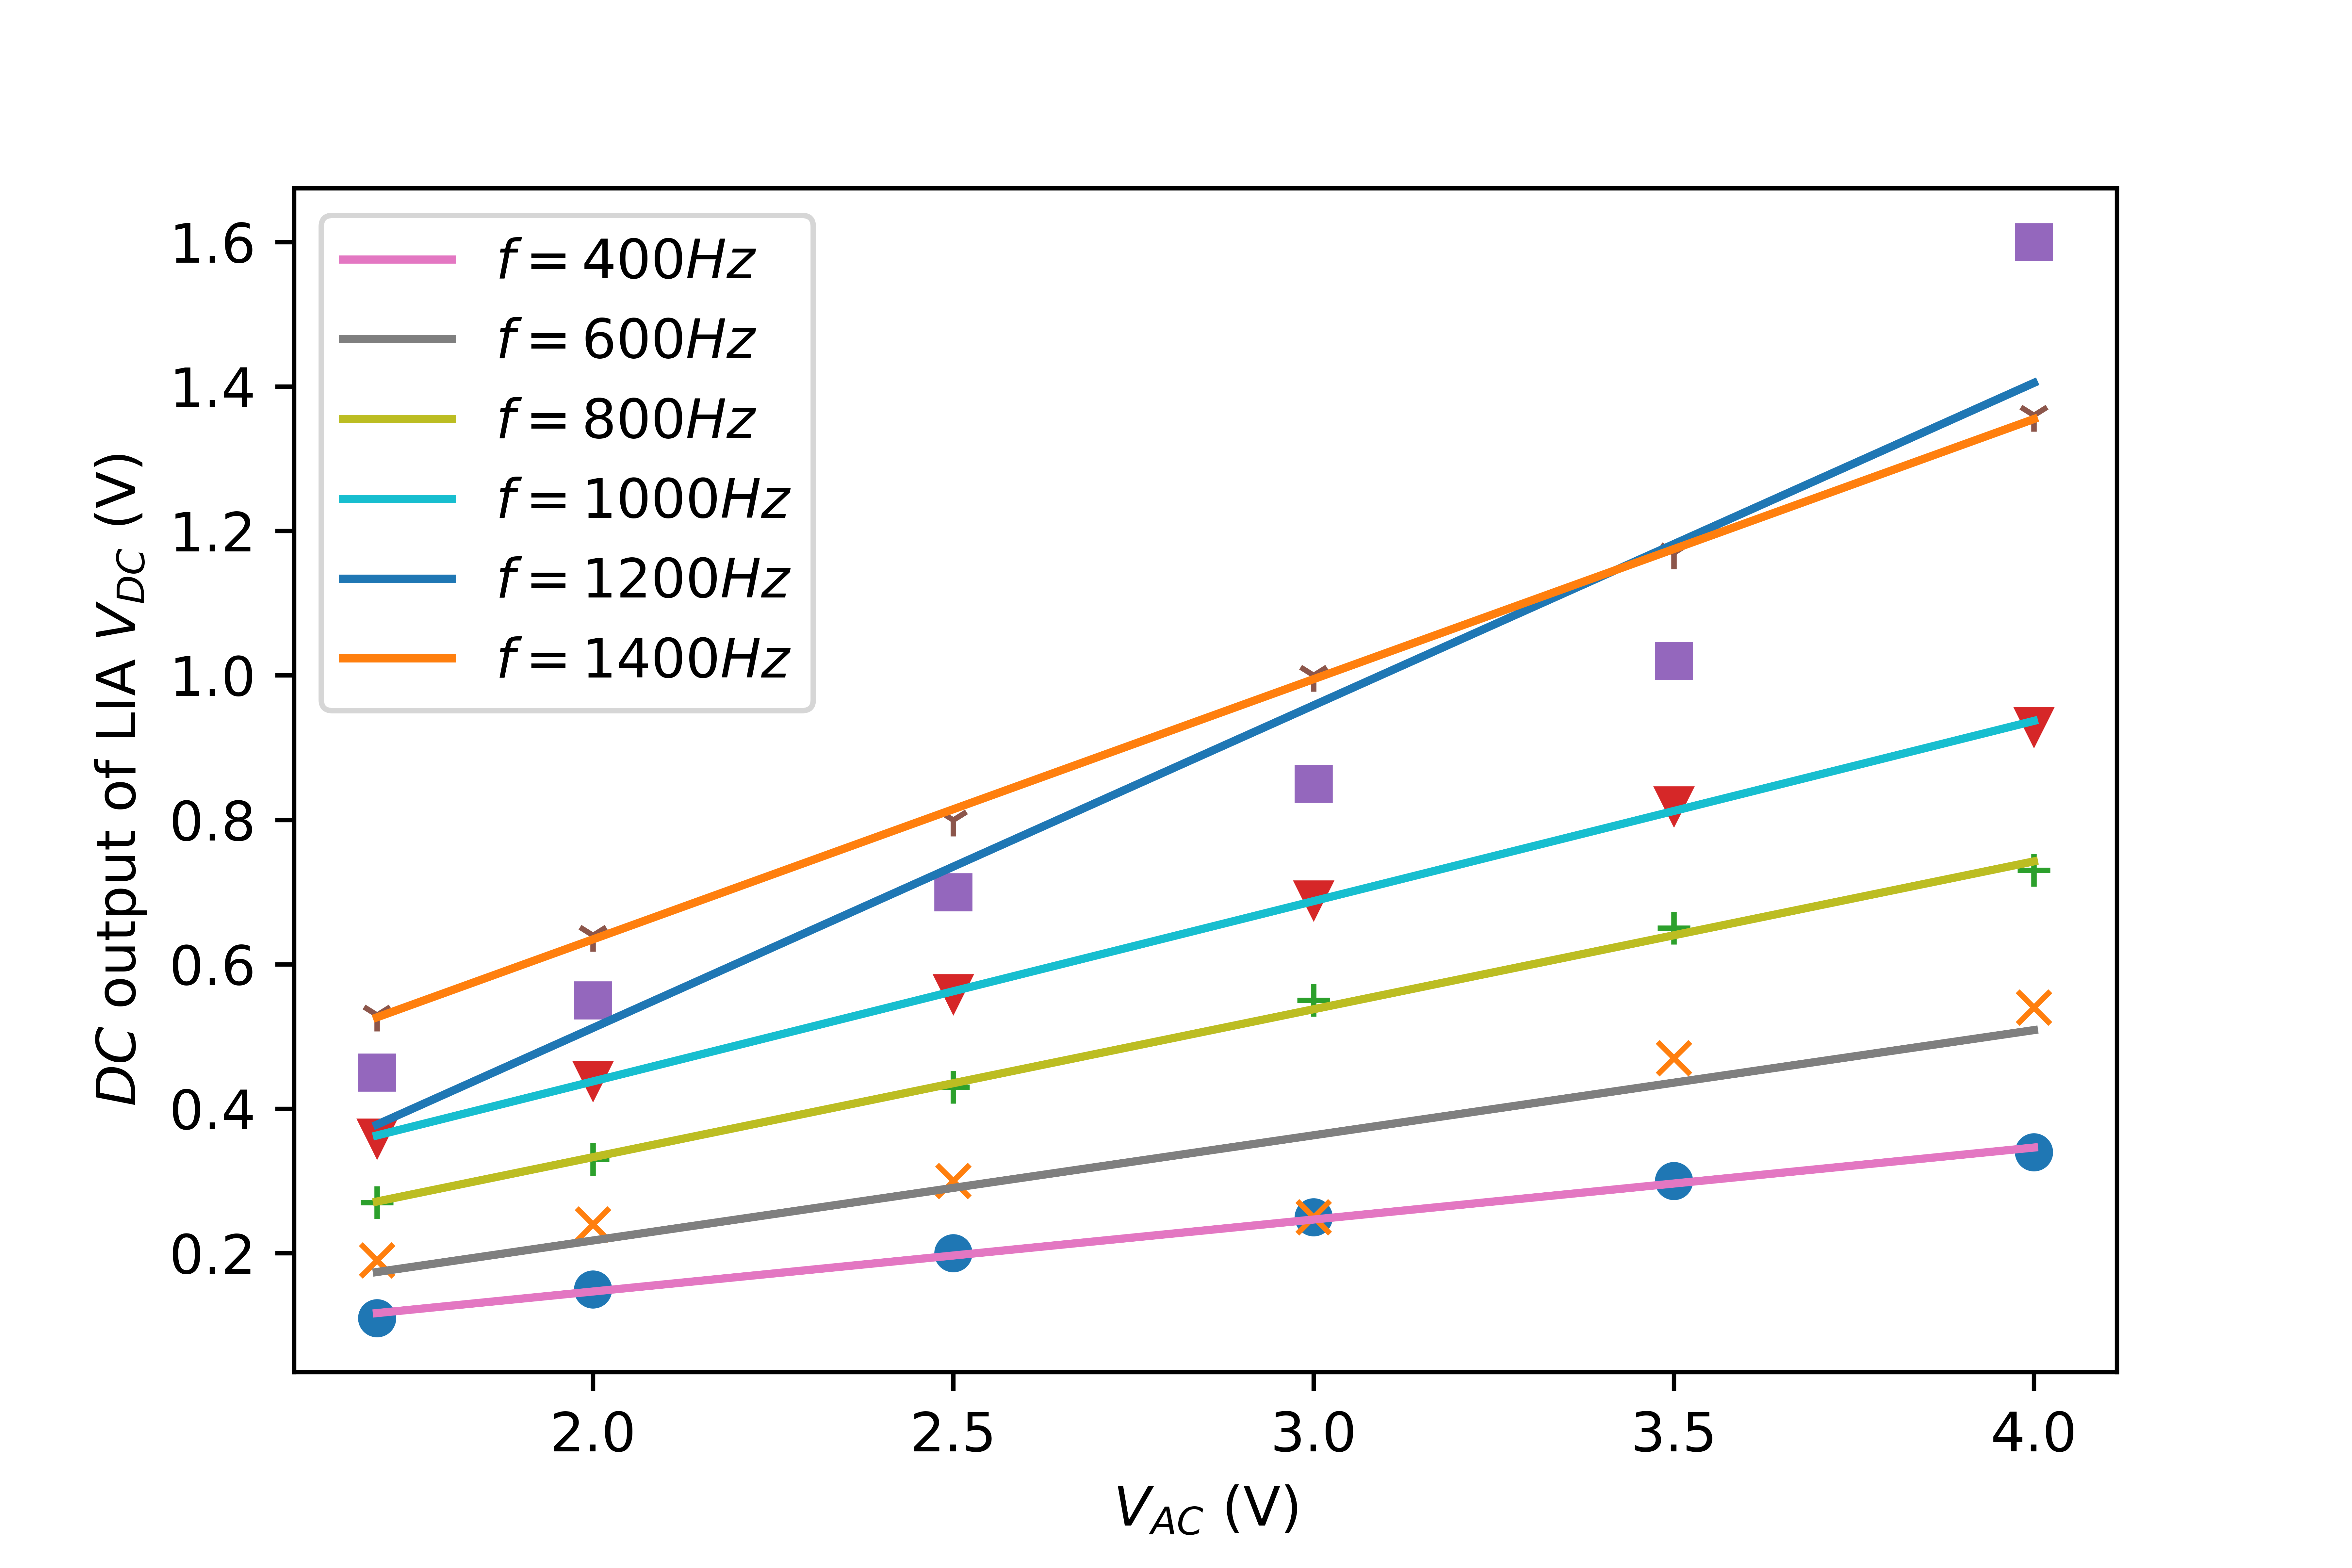
\includegraphics[scale = 0.56]{Figures/plot-mutinduct.png}
                \caption{$DC$ Output of LIA vs $AC$ voltage applied to primary circuit}
                \label{fig:mutinductplot}
            \end{figure}
        \subsubsection{Results}
            \begin{table}[]
            \caption{\label{tab:mutslope}Slopes of these curves at different frequencies}
            \centering
            \begin{tabular}{cc}
            \toprule
            \begin{tabular}[c]{@{}c@{}}Frequency $f$\\ (Hz)\end{tabular} & \begin{tabular}[c]{@{}c@{}}Slope $\alpha$ \end{tabular} \\
            \midrule
            400  & 0.0997 \\
            600  & 0.1456 \\
            800  & 0.2048 \\
            1000 & 0.2496 \\
            1200 & 0.4465 \\
            1400 & 0.3601 \\
            \bottomrule
            \end{tabular}
            \end{table}
            \begin{figure}
                \centering
                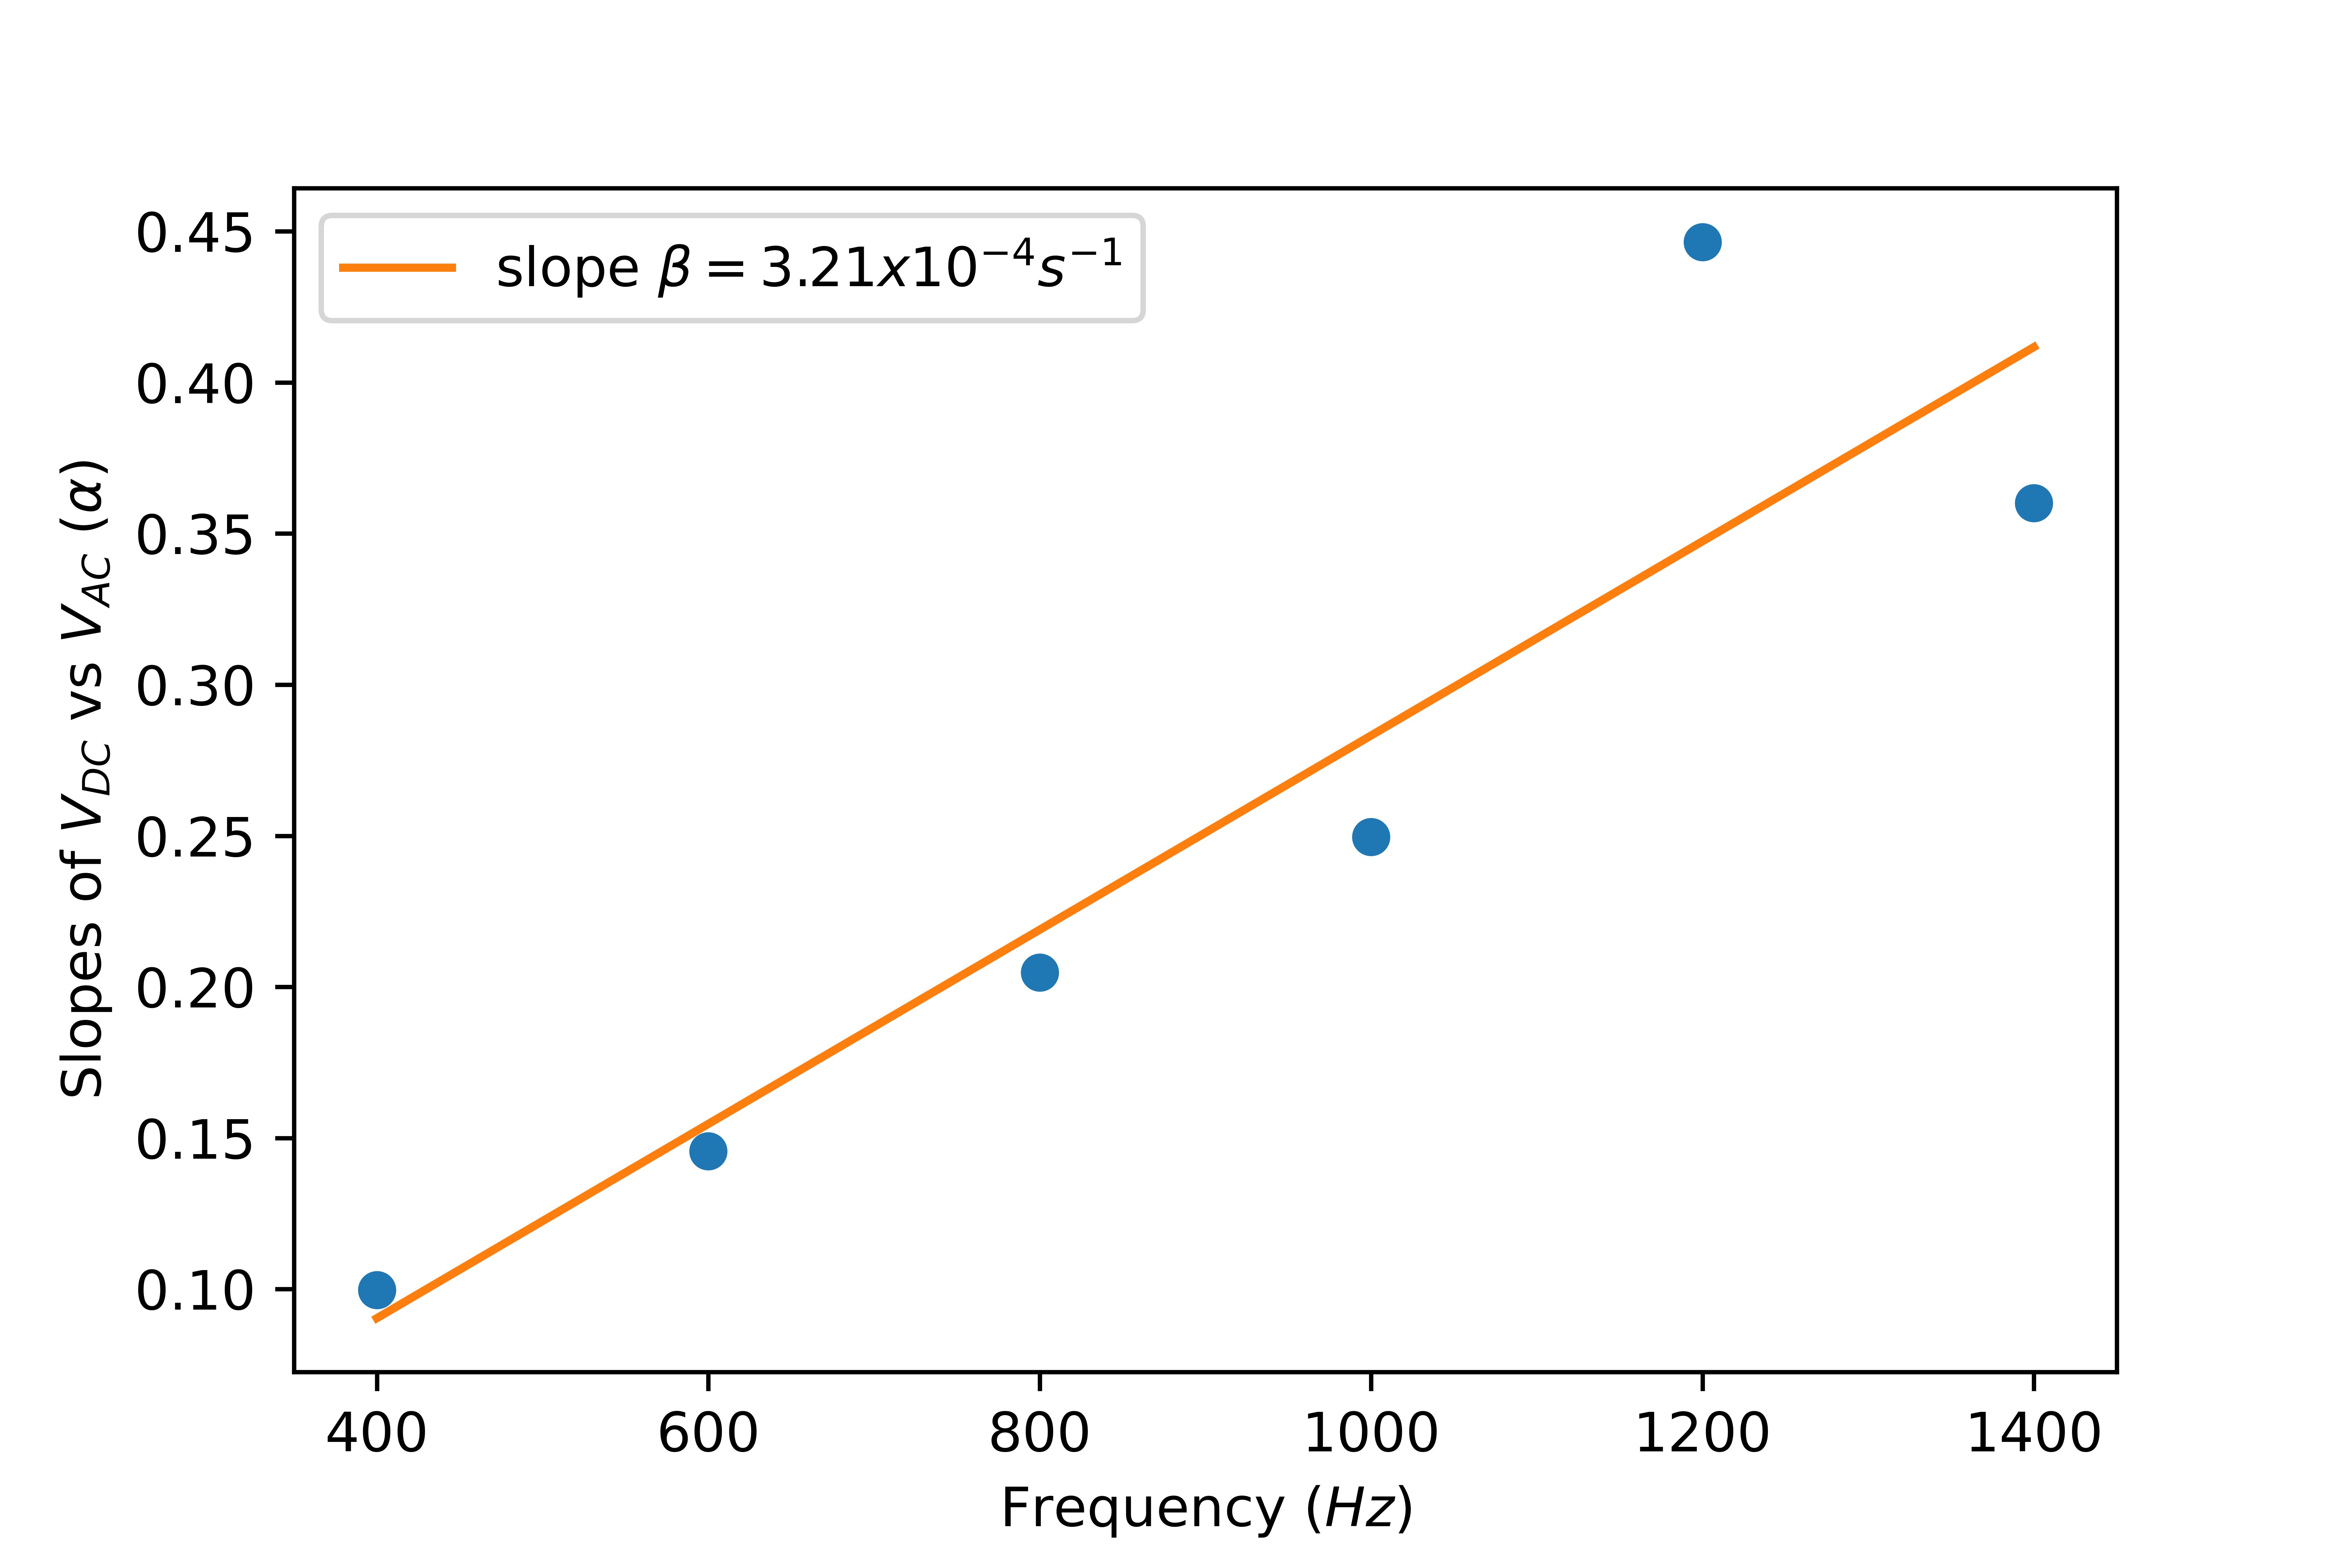
\includegraphics[scale = 0.56]{Figures/plot-mutslope.png}
                \caption{Slopes of $V_{DC}$ vs $V_{AC}$ from figure (\ref{fig:mutinductplot}) vs frequency}
                \label{fig:mutslope}
            \end{figure}
            Therefore, we see that the plot in figure (\ref{fig:mutslope}) is linear with a slope $\SI{3.21e-4}{\per \second}$. Figure (\ref{fig:mutinductplot}) show that the mutual inductance emf is proportional to the current through the primary coil, and figure (\ref{fig:mutslope}) to the frequency of the $AC$ current.
            \par
            The slope $\beta$ of the graph in figure (\ref{fig:mutslope}) must be equal to
            \begin{equation}
            \label{eq11}
                \beta = \dfrac{2 \pi M \mu}{R}
            \end{equation}
            where $M$ is the mutual inductance of the coil, $\mu$ is the amplification factor of the LIA and $R$ is the resistance in the primary circuit ($\SI{4.8}{\kilo \ohm}$). Average $\mu$ for the LIA is $1.53 \times 10^3$ from the data in table (\ref{tab:calibamp}). Putting these values in equation (\ref{eq11}), we get
            \begin{equation}
                \boxed{M \approx \SI{160.3}{\micro \henry}}
            \end{equation}
    \subsection{Measurement of low-resistance}
        Measurement of low resistance (resistance less than an Ohm) with the $DC$ technique would require a high current. Also since the voltage developed across the resistance will be small, it will be affected by noise when it is amplified.
        \par
        The AC technique using a lock-in-amplifier provides a solution to the problem as will be illustrated by this experiment.
        \par
        The apparatus required for this experiment is a signal generator, a lock-in amplifier, a two-channel oscilloscope, a low resistance box, one digital multimeter to measure $AC$ frequency and one digital multimeter to measure output of lock-in amplifier to two decimal places in the $DC$ $\SI{20}{\volt}$ range. 
        \subsubsection{The Low Resistance Box}
            In this box a resistance of $\SI{4.7}{\kilo \ohm}$ ($\SI{0.25}{\watt}$) is connected with the low resistance and a $\SI{100}{\ohm}$ ($\SI{0.25}{\watt}$) resistor. The free end of the $\SI{4.7}{\kilo \ohm}$ resistor is connected to the red banana terminal, the free end of the low resistance to the middle terminal (green). A $\SI{100}{\ohm}$ resistor is connected to the middle terminal (green) and the end terminal (in the figure (\ref{fig:resbox}) this terminal is yellow). Potential leads across the low resistance come to the $RCA$ socket marked \textit{signal} on the left top of the box. The voltage across the $\SI{100}{\ohm}$ resistor serves as the reference signal. This reference signal can be taken between the middle and end banana terminals on the box or from the $RCA$ socket marked \textit{reference} at the right top of the box. 
            \begin{figure}
                \centering
                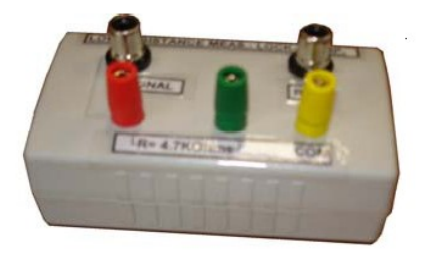
\includegraphics[scale = 0.7]{Figures/lowresbox.png}
                \caption{Low Resistance Box}
                \label{fig:resbox}
            \end{figure}
            \par
            The circuit diagram is as given in figure (\ref{fig:circuit}). The low resistance connected in the circuit is of less than $\SI{1}{\ohm}$.
            \begin{figure}
                \centering
                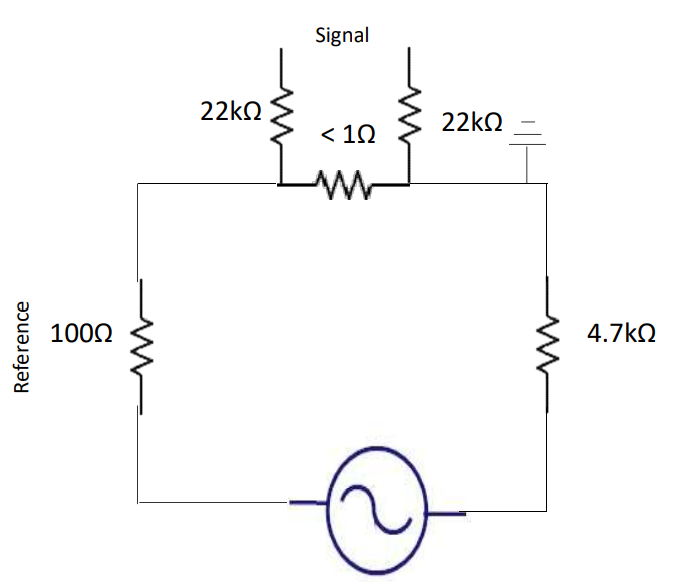
\includegraphics[scale = 0.6]{Figures/circuitlowres.png}
                \caption{Circuit diagram for the low resistance box experiment}
                \label{fig:circuit}
            \end{figure}
            \par
            The low resistance is made of insulated thin copper wire ($SW42$). One free end of the wire is soldered to the $\SI{4.7}{\kilo \ohm}$ resistor and the other free end to the $\SI{100}{\ohm}$ resistor. Two potential leads are soldered on the copper wire between the current leads. The free ends of the potential leads are soldered to the terminals of the $RCA$ socket marked \textit{signal}. The $\SI{4.7}{\kilo \ohm}$ resistor limits the current through the wire to a few hundred micro amperes when the signal generator output is connected to the terminals of the box.
        \subsubsection{Experimental Procedure}
            \begin{enumerate}
                \item The output terminals of the signal generator are connected to the two end banana terminals on the box. The reference signal, taken from the $RCA$ socket marked \textit{reference} is connected to the $RCA$ socket marked \textit{EXT REF} on the front panel of the lock-in amplifier.
                \item The $RCA$ socket marked \textit{signal} on the box is connected to the banana terminals marked \textit{EXT SIG} on the lock-in amplifier front panel.
                \item The socket marked \textit{output} on the front panel of the LIA is connected to a digital multimeter in the $DC$ $\SI{20}{\volt}$ range.
                \item The switches \textit{SW1} and \textit{SW2} on the LIA are put to the positions marked \textit{EXT} and the switch \textit{SW3} up.
                \item The signal generator is switched on and its frequency is adjusted to be about $\SI{200}{\hertz}$ and its amplitude about $\SI{4}{\volt}$ ($V_{AC}$).
                \item The lock-in amplifier is switched on and a \textit{DC} voltage appears on the digital multimeter which reaches a positive maximum value as the phase adjust pot is turned to the right extreme position. This maximum value of \textit{DC} voltage is noted as $V_{DC}$.
                \item The signal generator output $V_{AC}$ is changed in steps of $\SI{0.5}{\volt}$ down to $\SI{2}{\volt}$ and the voltage $V_{DC}$ is noted. The experiment is repeated at different frequencies in steps of $\SI{200}{\hertz}$.
                \item At each frequency, a graph between $V_{DC}$ and $V_{AC}$ is plotted. The points are fitted to a straight line and the slope \Bigg($\dfrac{d V_{DC}}{d V_{AC}}$ \Bigg) is obtained.
            \end{enumerate}
            Now, we have
            \begin{equation}
                d V_{AC} = R d I_{AC}
            \end{equation}
            where $R$ is the total resistance in the primary circuit ($\SI{4.8}{\kilo \ohm}$) and $d I_{AC}$ is the change in the current through the low resistance when the signal generator voltage is changed by $d V_{AC}$. The output \textit{DC} signal $V_{DC}$ is proportional to the voltage $V_r$ across the low resistance $r$. When the current through the low resistance is changed by $d I_{AC}$, the voltage $V_r$ changes by $d V_r$ where
            \begin{equation}
                d V_r = r d I_{AC}
            \end{equation}
            and this causes a change in $V_{DC}$ by $d V_{DC}$ given by
            \begin{equation}
                d V_{DC} = \mu d V_r = \mu r d I_{AC} = \Bigg( \mu \dfrac{r}{R} \Bigg) d V_{AC}
            \end{equation}
            So
            \begin{equation}
            \label{eq16}
                \dfrac{d V_{DC}}{d V_{AC}} = \Bigg( \mu \dfrac{r}{R} \Bigg) 
            \end{equation}
            \par
            To ensure that the contribution to $V_r$ from any residual inductance of the low resistance is small, we work at low frequencies and we check that the slope \Bigg($\dfrac{d V_{DC}}{d V_{AC}}$ \Bigg) is independent of the frequency. 
        \subsubsection{Observations}
            The readings obtained from the procedure for various frequencies are tabulated in table (\ref{tab:lowresbox}). The plot of $V_{DC}$ against $V_{AC}$ for each frequency are plotted in figure (\ref{fig:lowresplot}). The slopes of these curves at different frequencies are given in table (\ref{tab:lowresslope}).
            \begin{table}[]
            \caption{\label{tab:lowresbox} Readings for the low resistance box experiment with the lock-in amplifier}
            \centering
            \begin{tabular}{cccccccccccccc} \\ \toprule
            \multicolumn{2}{c}{$f = \SI{200}{\hertz}$} & \phantom{ab} & \multicolumn{2}{c}{$f = \SI{400}{\hertz}$} & \phantom{ab} & \multicolumn{2}{c}{$f = \SI{600}{\hertz}$} & \phantom{ab} & \multicolumn{2}{c}{$f = \SI{800}{\hertz}$} \\ \midrule
            \begin{tabular}[c]{@{}c@{}}$V_{AC}$\\ \scriptsize (V) \end{tabular} & \begin{tabular}[c]{@{}c@{}}$V_{DC}$\\ \scriptsize (V)\end{tabular} && \begin{tabular}[c]{@{}c@{}}$V_{AC}$\\ \scriptsize (V)\end{tabular} & \begin{tabular}[c]{@{}c@{}}$V_{DC}$\\ \scriptsize (V)\end{tabular} && \begin{tabular}[c]{@{}c@{}}$V_{AC}$\\ \scriptsize (V)\end{tabular} & \begin{tabular}[c]{@{}c@{}}$V_{DC}$\\ \scriptsize (V)\end{tabular} && \begin{tabular}[c]{@{}c@{}}$V_{AC}$\\ \scriptsize (V)\end{tabular} & \begin{tabular}[c]{@{}c@{}}$V_{DC}$\\ \scriptsize (V)\end{tabular} \\ \midrule
            2 & 0.27 && 
            2 & 0.27 && 
            2 & 0.28 &&
            2 & 0.28  \\
            2.5 & 0.35 && 
            2.5 & 0.34 && 
            2.5 & 0.35 && 
            2.5 & 0.34 \\
            3 & 0.39 && 
            3 & 0.41 && 
            3 & 0.43 && 
            3 & 0.42 \\
            3.5 & 0.46 && 
            3.5 & 0.49 && 
            3.5 & 0.49 && 
            3.5 & 0.48 \\
            4 & 0.56 && 
            4 & 0.55 && 
            4 & 0.56 &&
            4 & 0.55  \\
            \bottomrule
            \end{tabular}
            \end{table}
            \begin{figure}
                \centering
                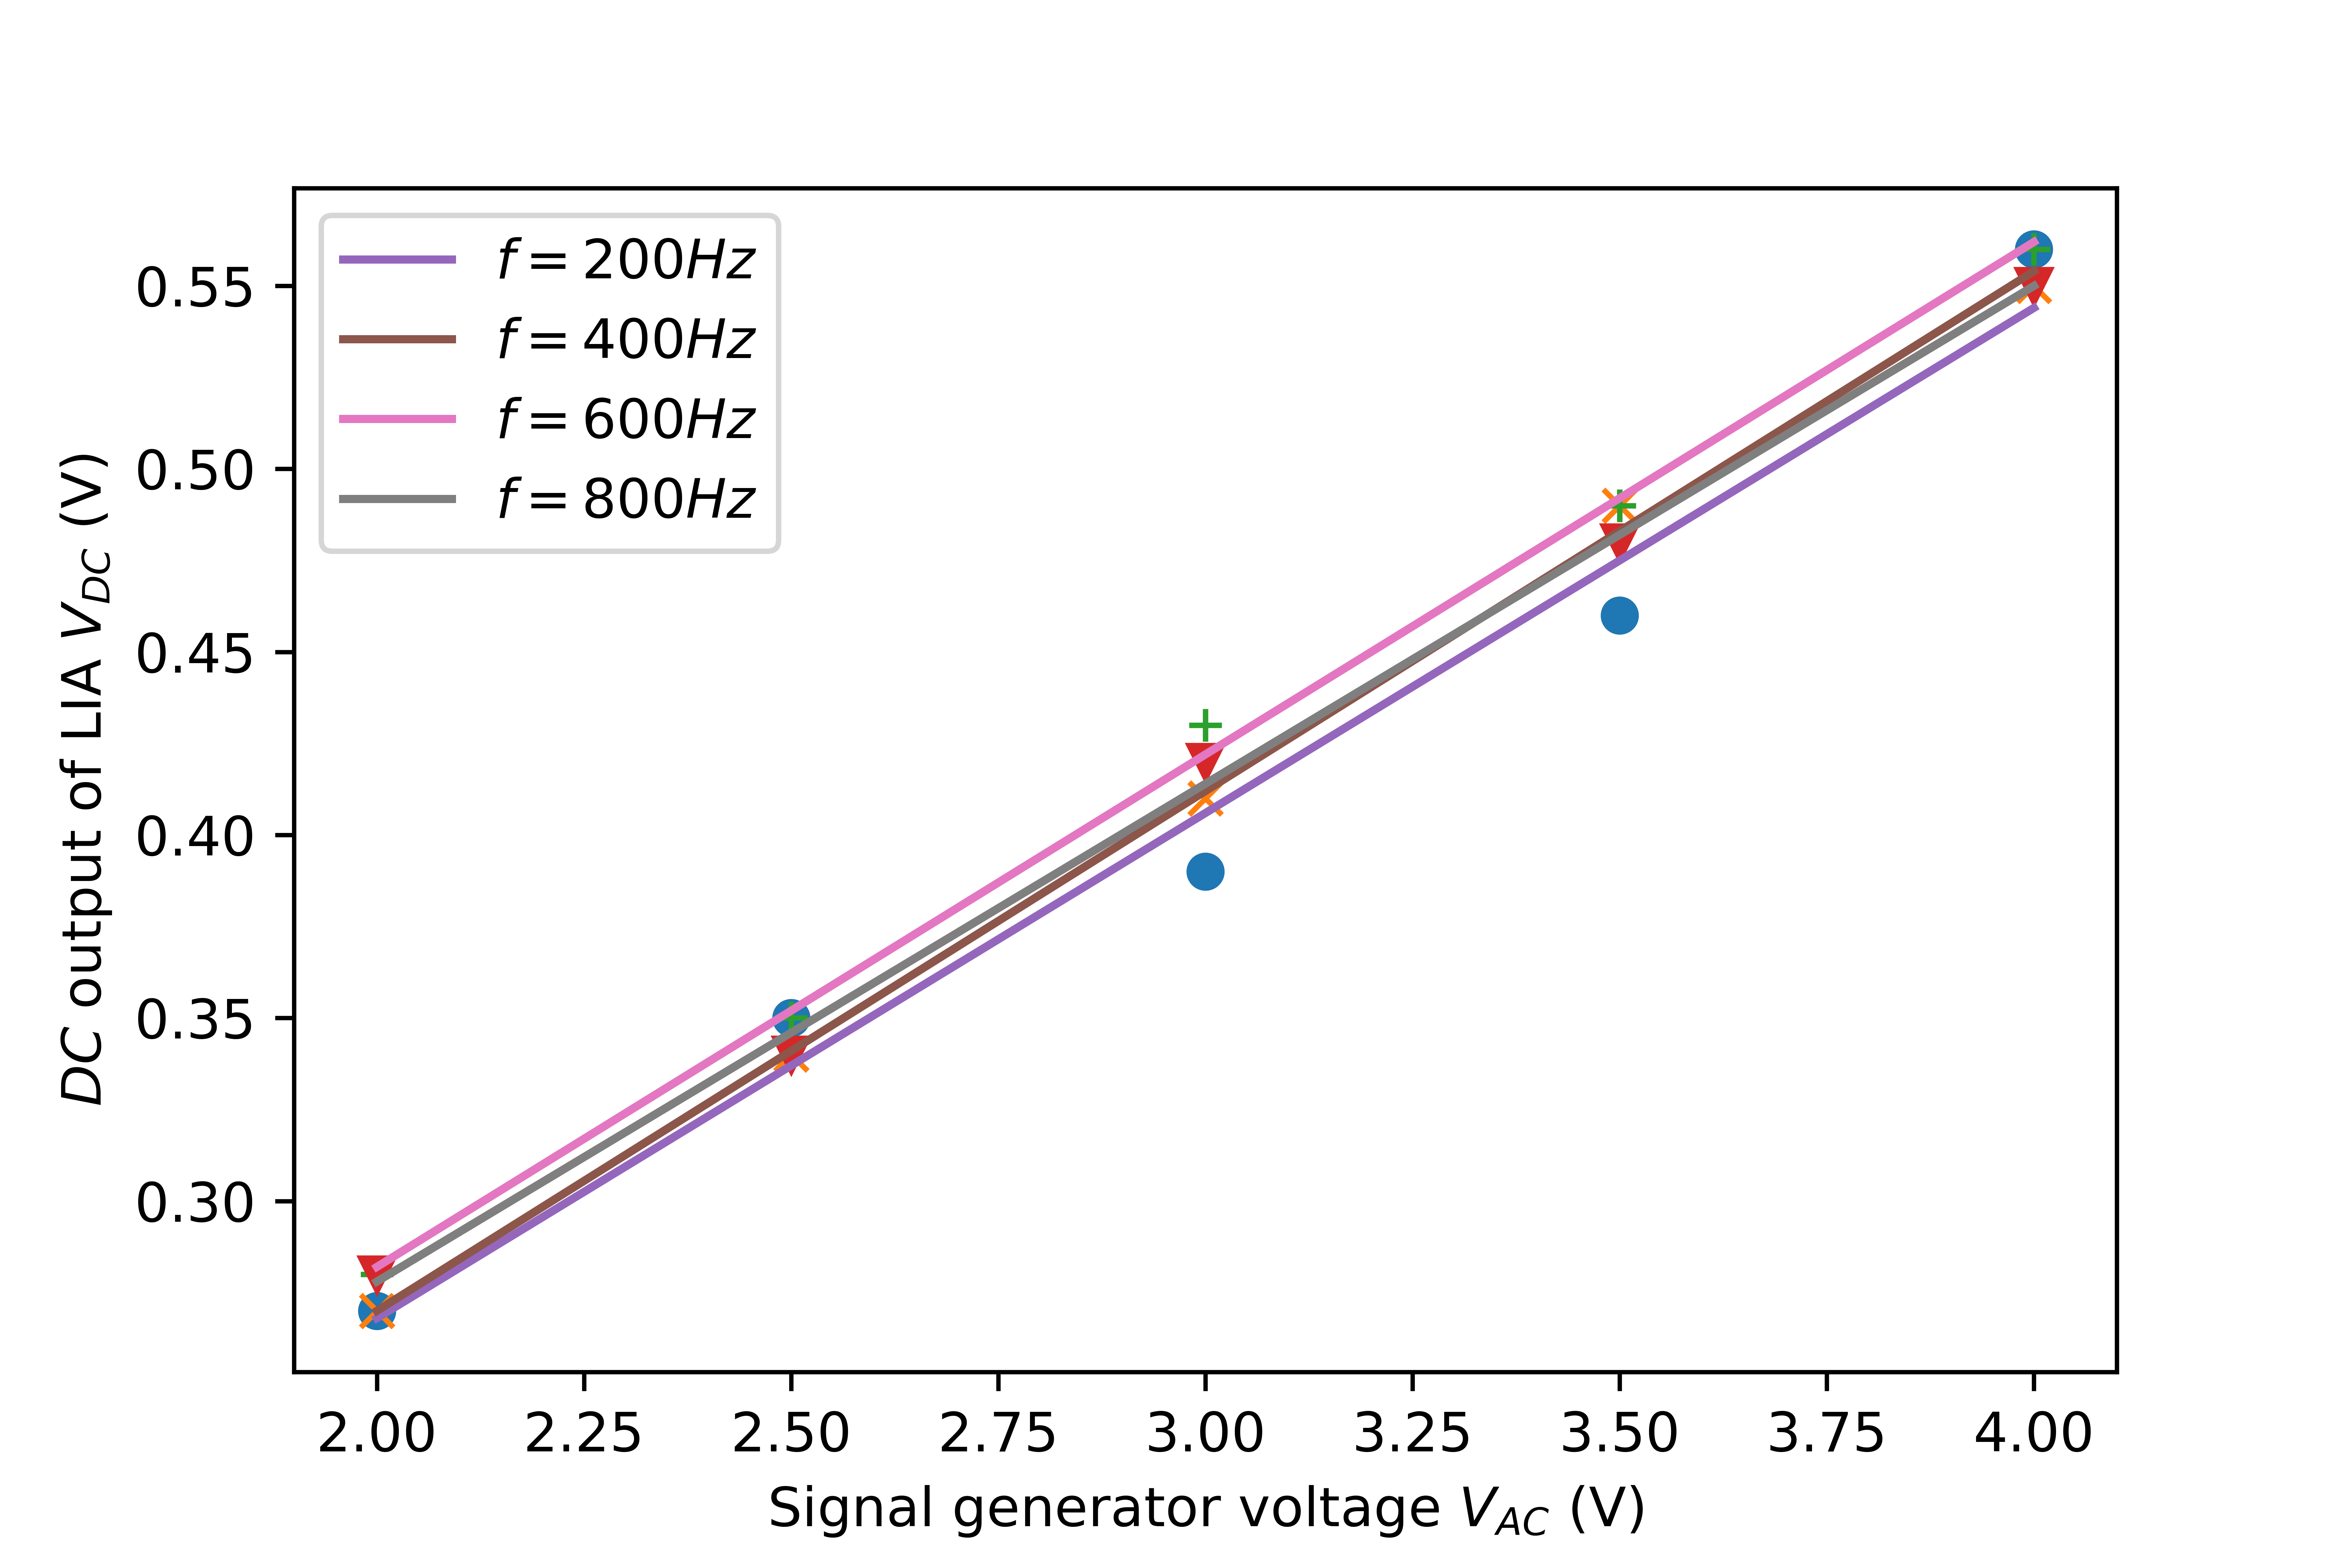
\includegraphics[scale = 0.56]{Figures/plot-lowresbox.png}
                \caption{$DC$ Output of LIA vs $AC$ voltage applied to primary circuit}
                \label{fig:lowresplot}
            \end{figure}
        \subsubsection{Results}
            \begin{table}[]
            \caption{\label{tab:lowresslope}Slopes of these curves at different frequencies}
            \centering
            \begin{tabular}{cc}
            \toprule
            \begin{tabular}[c]{@{}c@{}}Frequency $f$\\ (Hz)\end{tabular} & \begin{tabular}[c]{@{}c@{}}Slope $\alpha$\end{tabular} \\
            \midrule
            200 & 0.138 \\
            400 & 0.142 \\
            600 & 0.140 \\
            800 & 0.136 \\
            \bottomrule
            \end{tabular}
            \end{table}
            We see that the slope is nearly constant and is around $0.139$ (average value). From this average slope we can calculate the low resistance $r$ from the formula given in equation (\ref{eq16}). In that formula, (average) $\mu = 1.53 \times 10^3$ for the lock in amplifier used, $R = \SI{4.8}{\kilo \ohm}$. Substituting these values in the equation we find
            \begin{equation}
                \boxed{r = \SI{0.436}{\ohm}}
            \end{equation}
            



    

\section{Error Analysis}
    \subsection{Error in mutual inductance $M$}
        From equation (\ref{eq11}), we have
        \begin{equation}
            M = \dfrac{\beta R}{2 \pi \mu}
        \end{equation}
        To find error in $M$, we need errors in $\beta$ and $\mu$. Now, $\mu$ is the average amplification factor given by $\mu = 1.53 \times 10^3$. Now for the uncertainty in $\mu$, we will be calculating the standard deviation of the $\mu$ values in table (\ref{tab:calibamp}). Standard deviation of a sample is given by
        \begin{equation}
            \sigma = \sqrt{\dfrac{1}{N-1} \sum_{i=1}^{N} (x_i - \bar x)^2}
        \end{equation}
        From here, we get uncertainty in $\mu$ as $0.03 \times 10^3$. Now, note that $\beta$ is the slope in the figure (\ref{fig:mutslope}). Therefore, we need to calculate error in slope which is given by
        \begin{equation}
        \label{eq20}
            \sigma_m = \sigma_y \times \sqrt{\dfrac{S}{\Delta}}
        \end{equation}
        where $S$ is the number of observations (which is 6) and $\Delta = S \Sigma x^2 - (\Sigma x)^2 = \SI{4.2e6}{\second}$. Note that $\sigma_y$ is the uncertainty in the slopes found from the plot $V_{DC}$ against $V_{AC}$ for different frequencies. The uncertainty in $y$ values, that is, in values of $V_{DC}$ in figure (\ref{fig:mutinductplot}) is the least count which is equal to $\SI{0.01}{\volt}$. Using equation (\ref{eq20}), we have $\sigma_y = 5.05 \times 10^{-3}$. From this, we get the error in $\beta$ as $6.04 \times 10^{-6}$. Therefore we have
        \begin{equation}
            \label{eq21}
            \mu = (1.53 \pm 0.03) \times 10^3
        \end{equation}
        and
        \begin{equation}
            \beta = (3.21 \pm 0.06) \times 10^{-4}
        \end{equation}
        Now, error in $M$ is given by
        \begin{equation}
            dM = \sqrt{\Big(\dfrac{\partial M}{\partial \beta} \sigma_{\beta}\Big)^2 + \Big(\dfrac{\partial M}{\partial \mu} \sigma_{\mu}\Big)^2}
        \end{equation}
        Putting in the values, we get
        \begin{equation}
            dM = \SI{4.34}{\micro \henry}
        \end{equation}
        Hence, we have
        \begin{equation}
            \boxed{M = \SI[separate-uncertainty=true]{160 \pm 4}{\micro \henry}}
        \end{equation}
    
    \subsection{Error in low resistance $r$}
        From equation (\ref{eq16}), we have
        \begin{equation}
            r = \dfrac{m R}{\mu}
        \end{equation}
        where $m = \dfrac{d V_{DC}}{d V_{AC}}$. To find error in $r$, we need errors in $m$ and $\mu$. We have already found the uncertainty in $\mu$ as in equation (\ref{eq21}). Now as $m$ is the slope of the curves in figure (\ref{fig:lowresplot}), we take the average value of $m = 0.139$ and the uncertainty would be given by the standard deviation in the values of $m$ and is equal to 0.003. Now error in $r$ is given by
        \begin{equation}
            dr = \sqrt{\Big(\dfrac{\partial r}{\partial m} \sigma_{m}\Big)^2 + \Big(\dfrac{\partial r}{\partial \mu} \sigma_{\mu}\Big)^2}
        \end{equation}
        Putting in the values, we get
        \begin{equation}
            dr = \SI{0.013}{\ohm}
        \end{equation}
        Thus
        \begin{equation}
            \boxed{r = \SI[separate-uncertainty=true]{436 \pm 13}{\milli \ohm}}
        \end{equation}



\section{Discussions}
\begin{enumerate}
    \item Signal recovery takes advantage of the fact that noise is often spread over a much wider range of frequencies than the signal. In the simplest case of white noise, even if the root mean square of noise is $10^3$ times as large as the signal to be recovered, if the bandwidth of the measurement instrument can be reduced by a factor much greater than $10^6$ around the signal frequency, then the equipment can be relatively insensitive to the noise.
    \item In a typical $\SI{100}{\mega \hertz}$ bandwidth (e.g. an oscilloscope), a band-pass filter with width much narrower than $\SI{100}{\hertz}$ would accomplish this. The averaging time of the lock-in amplifier determines the bandwidth and allows very narrow filters, less than $\SI{1}{\hertz}$ if needed. However, this comes at the price of a slow response to changes in the signal.
    \item In summary, even when noise and signal are indistinguishable in the time domain, if the signal has a definite frequency band and there is no large noise peak within that band, noise and signal can be separated sufficiently in the frequency domain.
    \item When the lock-in technique is applied, care must be taken to calibrate the signal, because lock-in amplifiers generally detect only the root-mean-square signal of the operating frequency. For a sinusoidal modulation, this would introduce a factor of $\sqrt{2}$ between the lock-in amplifier output and the peak amplitude of the signal, and a different factor for non-sinusoidal modulation.
    \item In the case of nonlinear systems, higher harmonics of the modulation frequency appear. A simple example is the light of a conventional light bulb being modulated at twice the line frequency. Some lock-in amplifiers also allow separate measurements of these higher harmonics.
    \item Furthermore, the response width (effective bandwidth) of detected signal depends on the amplitude of the modulation. Generally, linewidth/modulation function has a monotonically increasing, non-linear behavior.
    \item To summarise the working principle of the lock-in amplifier, the lock-in is supplied with a reference input sinusoidal voltage that is synchronized with the main signal whose amplitude is being measured. The lock-in uses this reference signal to find the signal to be measured, while ignoring anything that is not synchronized with the reference. The principle employed here is of phase sensitive detection (PSD).
    \item The mutual inductance directly depends on the number of turns in the coils. It is inversely proportional to the length of the coils.
    \item The mutual inductance decreases when the separation between the two coils is increased as the flux linked with the secondary due to the current in the primary, decreases.
    \item From equation (\ref{eq9}), it is clear that if the frequency of the signal is decreased, the induced emf in the secondary for the same current in the primary will decrease (in magnitude).
    \item In the low resistance part of the experiment, we note that the residual inductance of the low resistance was not considered. If considered, there would be slight modifications in our calculations.
\end{enumerate}

\section{Conclusions}
\begin{enumerate}
    \item The value of mutual inductance $M$ was found to be $M = \SI[separate-uncertainty=true]{160 \pm 4}{\micro \henry}$.
    \item The value of small resistance $r$ was found to be $r = \SI[separate-uncertainty=true]{436 \pm 13}{\milli \ohm}$.
    \item While calibrating the lock-in amplifier, the slope of the plots of $V_{DC}$ against $V_{sig}$ remains constant with increase in frequency (figure (\ref{fig:calibdata})).
    \item In the mutual inductance part of the experiment, the slopes of the plots of $V_{DC}$ against $V_{AC}$ increase with the increase in frequency (figure (\ref{fig:mutinductplot})).
    \item The mutual inductance emf is $90 \degree$ out of phase with the current in the primary coil. It is proportional to the current in the primary coil and to the frequency. 
    \item In the row resistance part of the experiment, the slope of the plots of $V_{DC}$ against $V_{AC}$ remains constant with increase in frequency (figure (\ref{fig:lowresplot})). 
    \item The lock-in amplifier was calibrated and after that mutual inductance of two coils and the value of small resistance was determined. The results so obtained were in the order of the expected values. The experiment was thus a success.
\end{enumerate}




% Produces the bibliography via BibTeX.

\end{document}
%
% ****** End of file apssamp.tex ******
